\documentclass[12pt,oneside,a4paper]{article}
\usepackage{lmodern}
\usepackage[utf8]{inputenc}		% Codificacao do documento (conversão automática dos acentos)
\usepackage[english]{babel}
\usepackage[T1]{fontenc}
\usepackage{amsmath, amsfonts, amssymb}
\usepackage{graphicx}
\usepackage[left=2.00cm, right=2.00cm, top=2.00cm, bottom=2.00cm]{geometry}
\usepackage{setspace}
\usepackage{natbib}
%\usepackage{uarial}
%\usepackage{rotating,booktabs}
%\usepackage{inslrmin, pxfonts} 
%\usepackage{caption}
\usepackage{fancyhdr}   %cabeçalho com nome da seçao em cima
\setlength{\headheight}{15pt} % Correcao para \headheight
%\usepackage{lmodern}
\usepackage{microtype}
\usepackage{booktabs}
\usepackage[none]{hyphenat}
\usepackage{float}
\usepackage{mathrsfs}
\usepackage{indentfirst}		% Indenta o primeiro parágrafo de cada seção.
\usepackage{nomencl} 			% Lista de simbolos
\usepackage{color}				% Controle das cores
\usepackage{graphicx}			% Inclusão de gráficos
\usepackage{microtype} 			% para melhorias de justificação
%\usepackage[pdftex]{hyperref}  %para adicionar enderecos de internet
\usepackage{calrsfs}
\usepackage{float}
\usepackage{array}
%\definecolor{maroon}{RGB}{153, 0, 0}
\definecolor{brandeisblue}{rgb}{0.0, 0.44, 1.0}
\usepackage[colorlinks=true, linkcolor= black, citecolor=brandeisblue]{hyperref}


%%%%%%%%%%%%%%%%%%%%%%%%%%%%%%%%%%%%
%%%%%%%%%%%%%%%%%%%%%%%%%%%%%%%%%%%%

\title{Measuring the Natural Rate of Interest in Brazil and identifying its drivers: a DSGE Perspective}
\author{ Renan Alves\thanks{PhD candidate at the Sao Paulo School of Economics Fundação Getulio Vargas (FGV EESP). E-mail:  renan.salves29@gmail.com.}}
%\author{Renan Alves}
%\thanks{Ph.D. student at Sao Paulo School of Economics - FGV}
\date{}

\begin{document}

\maketitle

%%%%%%%%%%%%%%%%%%%%%%%%%%%%%%%%%%%%
%%%%%%%%%%%%%%%%%%%%%%%%%%%%%%%%%%%%

\begin{abstract}
   Digitar um texto aqui!!

	\noindent
	\\
	\textbf{Keywords:} Natural Interest Rate, Monetary Policy, Open Economy, Bayesian Estimation, Emerging Market
	
\end{abstract}

\onehalfspacing
%
%
\newpage
%
%
\section{Introduction}
The interest rate is the main instrument of monetary policy. The policymakers to assess monetary policy stance monitor what we call the natural rate of interest. The natural rate of interest  is the real interest rate at which the output is equal to its potential level, and prices neither accelerate nor decelerate. Therefore, the natural rate is a benchmark, since when it is above real interest, monetary policy was contractionary, and when it is below real interest, it was expansionary. The difficulty in monitoring this interest rate is that it cannot be observed and so it must be estimated. 

A decade later, the global financial crisis (GFC), the world economy remains sunk in a low interest rate environment amid the unconventional monetary policies implementation promoted by advanced economies, which drew attention to the natural rate of interest. The literature also found evidence for a historical decline and even negative levels in the natural rate in advanced economies over the last two decades, according to \citet{HLW:2017}, \citet{Wynne:2018}, and \citet{DelNegro:2019}.\footnote{\citet{HLW:2017}, using a semi-structural model, and \citet{DelNegro:2019}, through an vector autoregression (VAR), both find a downward trend in natural rates for advanced economies. \citet{Wynneb:2018} find the same result for a larger set of countries. }  
This economic environment is called secular stagnation, as \citet{Summers:2014} characterizes it, because of low interest rates and low growth. Some studies to explain the reasons for the fall in interest rates, such as preferences for safe assets \citet{Caballero:2017} and demographic causes \citet{Eggertsson:2019}.

The unconventional monetary policy strategies adopted by the advanced economies in response to the GFC provoked a flood of capital flow towards the emerging economies. The result was rapid credit growth, which has required many emerging countries to adjust their monetary policy to reduce the risks of financial instability and volatility in capital flow. This raises major concerns for policymakers because the capital flow affects the business cycle in emerging countries, \citet{Uribe:2016} and \citet{Cuadra:2019}. 


There are few studies that investigate the effects of capital flow on the  natural rate in emerging markets. \citet{Carrillo:2018} examine how Mexico's capital flow explains the drop in the natural rate of interest  after the global financial crisis. What we already know is that international interest and country spread shocks are drivers of business cycles in emerging economies, according to \citet{Uribe:2006}. These international factors are also important to explain the natural rate in emerging markets. \citet{Barbosa:2016} showed that the Brazilian natural rate can be explained by the international real interest rate and the country risk premium. 


%A stylized fact of the Brazilian economy was the high real interest rate. \citet{SEGURA-UBIERGO:2012} lists some arguments that try to explain why, for many years, Brazil's real interest was higher compared to that of other emerging countries. The combination of high levels of public debt and the fear of a possible default resulted in higher interest rates and an increased risk premium. The low savings rate is a limiting factor for economic growth and, therefore, a reason for higher interest rates. Third, the institutional weakness that creates legal uncertainty by not protecting investors. The presence of public banks offering credit at below-market rates affects the transmission mechanism of monetary policy since the rest of the economy's equilibrium interest rate needs to be higher to keep credit demand under control at a level consistent with the inflation targeting regime.

Brazil's monetary policy is often cited as excessively conservative, evidenced by one of the highest real interest rates among emerging economies.\footnote{A stylized fact of the Brazilian economy was the high real interest rate. \citet{SEGURA-UBIERGO:2012} lists some arguments that try to explain why, for many years, Brazil's real interest was higher compared to that of other emerging countries: The combination of high levels of public debt and the fear of a possible default, the low savings rate is a limiting factor for economic growth, the institutional weakness that creates legal uncertainty by not protecting investors and the presence of public banks offering credit at below-market rates affects the transmission mechanism of monetary policy.} However, as shown in figure 1, Brazil's real interest rate (measured as the nominal short-term interest rate (Selic) minus the expected inflation) has shown a downward trend in the last 18 years (figure on the left). The lowest real interest level was observed in December 2019, while the highest value was observed in July 2003. One reason why economists justify that Brazilian real interest rates were high is the high rate of inflation and volatility. Brazil adopted the inflation targeting regime in June 1999, and, as shown in the figure on the right, we can see that the inflation rate, measured by the consumer price index (CPI), was within the band for most of the years.\footnote{In January 1999, Brazil adopted the floating exchange rate regime, following emerging countries' trends at that time. Between the end of 2002 and the beginning of 2003, with the presidential election and the insecurity of adopting controversial economic measures, the country's risk increased, and the interest rate accompanies this movement.}


\begin{figure}[H]
\centering
\caption{Real interest and inflation in Brazil}
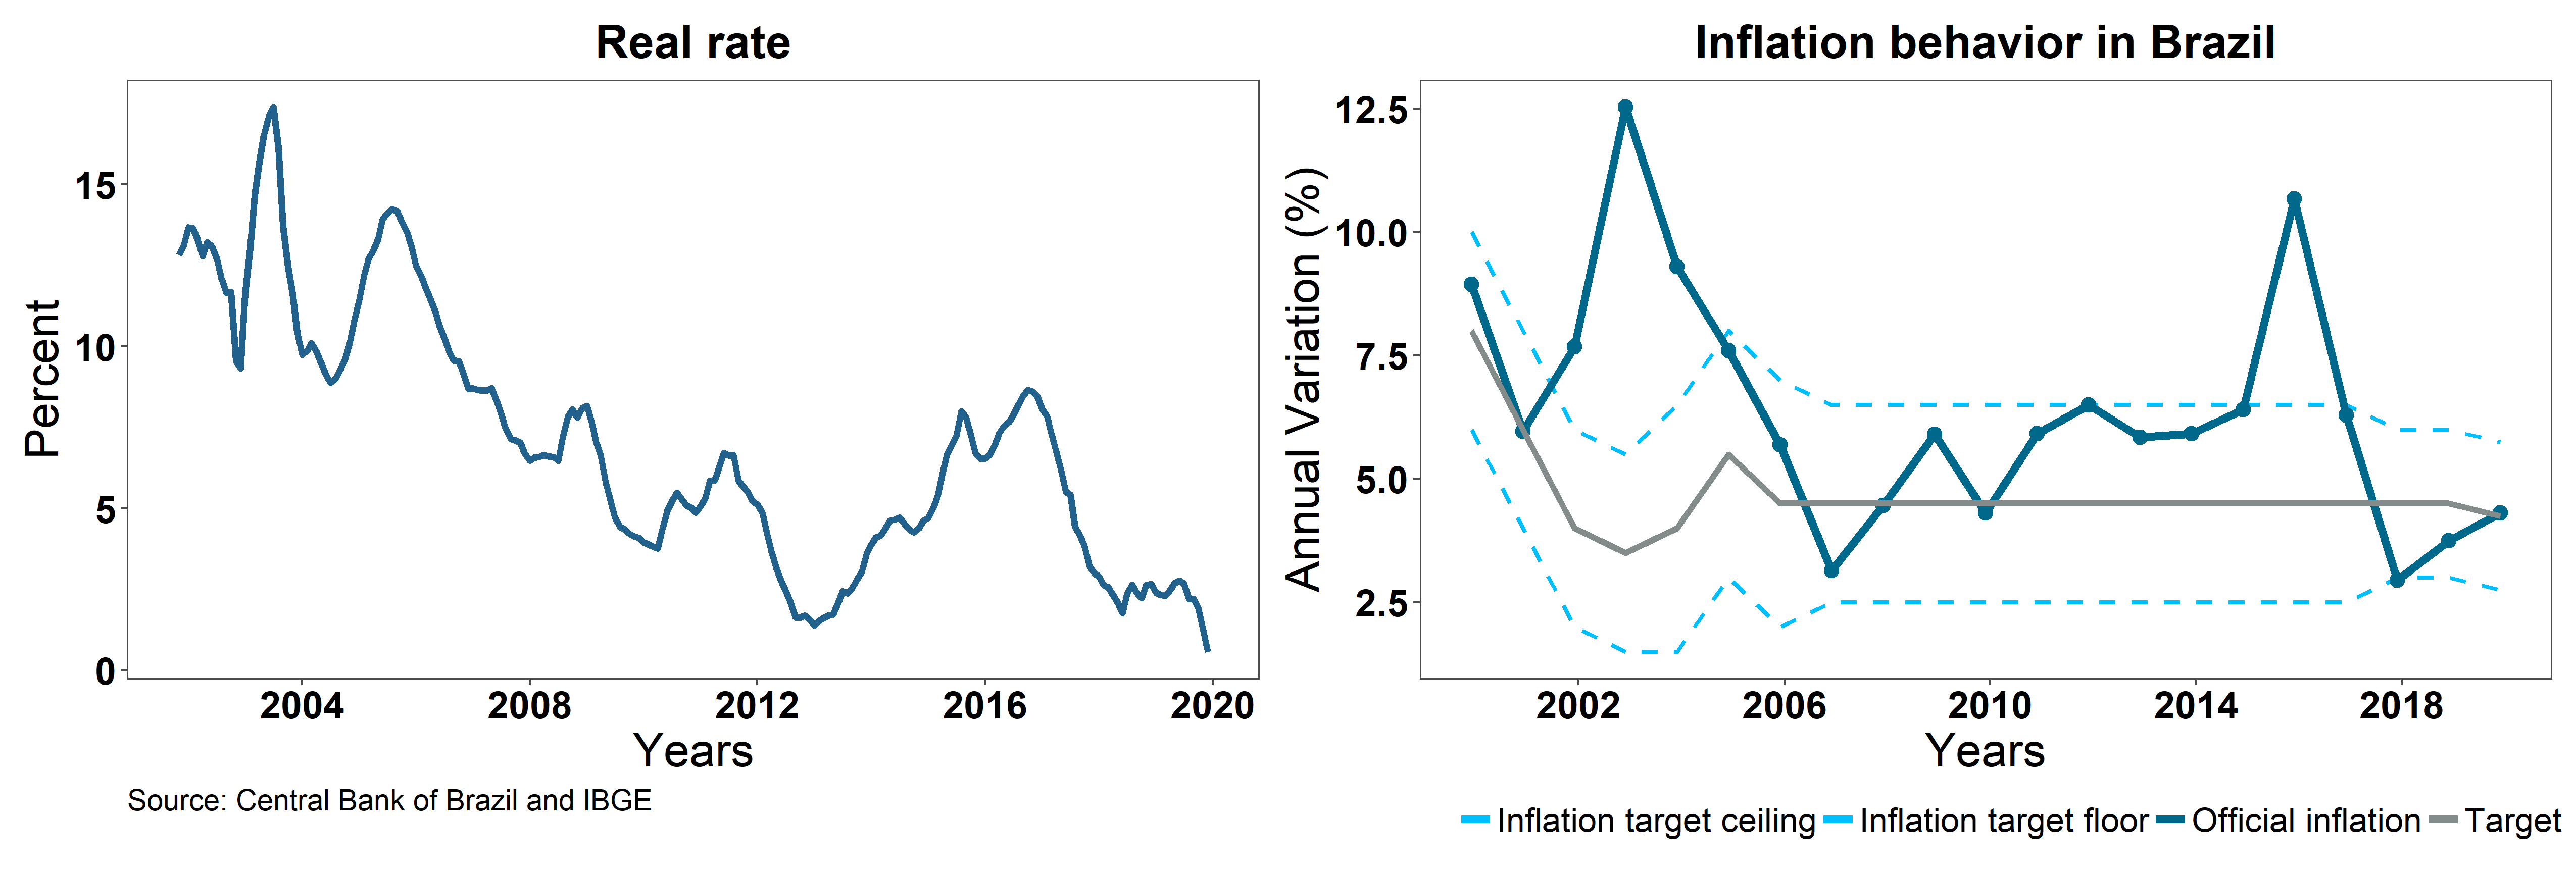
\includegraphics[scale=0.42]{Capitulo_1/Juros_inflacao.png}

\end{figure}



%Given this scenario in which interest rates in advanced economies are stuck in the zero lower bound, the emerging economies suffer from international interest rate and risk premium shocks and the fall in real rates in Brazil reaching the lowest level in 20 years, in this paper I estimate an open economy DSGE model based on \citet{Adolfson:2007} to answer the following questions: (i) what the level of Brazil's natural rate of interest  between 1999 and 2019; (ii) is will the natural rate have also declined as well as in advanced economies; (iii) what are the mechanisms that explain the Brazilian natural rate; (iv) whether external shocks are fundamental to explain the balance interest. According to \citet{Woodford:2003}, the natural rate of interest is the interest rate that would prevail if all prices and wages were flexible.

Given this secular stagnation scenario, represented by a downward trend in the real world interest rate and low growth rates in advanced economies, it is interesting to know whether in emerging economies the natural rate of interest  is also falling and whether this low interest rate global environment contributed to this fall. 

In this paper, we estimate a medium-scale New Keynesian open economy dynamic stochastic general equilibrium (DSGE) model using Bayesian techniques on Brazil data to answer the following questions: (i) what the level of Brazil's natural rate of interest  between 1999 and 2019; (ii) whether the natural rate have also declined as well as in advanced economies; (iii) what are the mechanisms that explain the Brazilian natural rate; (iv) whether international shocks are fundamental to explain the equilibrium rate. We follow \citet{Woodford:2003}, the natural rate of interest corresponds to the value of the real interest rate that would be realized if prices and wages are flexible, and absent shocks to the mark-ups on goods and labor markets.



%Few studies investigate whether the natural rate has also fallen in emerging countries, given this scenario in which interest rates in advanced economies have reached the lower limit of zero, and many papers have found evidence for the fall in natural interest in these countries.



We use a structural (DSGE) model in the same way as \citet{Neiss:2003} because this is an approach that has the advantage of providing an economic insight into the drivers of the natural rate. The model used in the analysis is a small open economy follows closely \citet{Adolfson:2007}, which is an extended open economy version of \citet{Christiano:2005} with both nominal and real frictions and \citet{Altig:2011}, who introduce a stochastic unit-root technology shock, which enables us to work with trending data.\footnote{It is a medium-scale version of the open economy models such as \citet{Gali:2005}, \citet{Monacelli:2005} and \citet{Lubik:2007}.} However, the model differs from \citet{Adolfson:2007} in four aspects.\footnote{This DSGE model, called RAMSES, used to forecasting and policy analysis at the Sveriges Riskbank, \citet{Adolfson:2008}.} First, households do not receive utility from holding cash. Second, we allow inflation in Brazil to be higher than inflation in the rest of the world. This allows for a differential in inflation rates, causing a depreciation of the nominal exchange rate at a steady state, which is in line with that predicted by the purchasing power parity theory. In monetary policy rule, the central bank responds to deviations of the output gap, defined as the difference between the actual and potential output. We define the potential output as the level of output that would prevail under flexible prices and wages in the absence of the “cost-push” shocks. Finally, the role of fiscal policy is disregarded in this model.

%The central bank's decision to raise or lower the short-term interest rate may have a material effect on the economy. This decision may affect inflation, unemployment, exchange rates and output growth. Due to the importance of setting interest rate, understanding where the natural rate is vital to making effective policy decisions. This becomes even more relevant for the Brazilian economy, given the enormous challenges and uncertainties arising from the fiscal issue, the local political scenario and international factors.

%I should note, however, that DSGE models generally estimate the business-cycle frequency component in the natural rate of interest . This is different from pure time-series models and from the semi-structural methods that, in turn, focus on low-frequency movements of the natural rate. However, the existing studies in the DSGE literature tend to estimate the natural rate of interest  within a closed-economy setup and only for large economies such as the U.S., the euro area, and Japan.


%
%
\section{Literature Review}
In the past two decades, various papers have proposed approaches to estimate the unobservable natural rate of interest. This literature can be broadly divided into three strands, following \citet{Giammarioli:2004}: pure time series methods, semi-structural econometrics methods and structural methods.\footnote{For a useful review of the results found in the literature, see \citet{Brand:2018}. } It is worth mentioning that according to \citet{Wieland:2018}, there are three different concepts of the natural rate and this differentiation depends on the time horizon, short-term, medium-term and long-term.\footnote{The first concept of equilibrium rate refers to that of short-term equilibrium and is often used in DSGE models. The second concept of the neutral interest rate in the medium-term, used in the semi-structural models introduced by \citet{LW:2003}. And the third concept is the long-term equilibrium rate. In DSGE models, the long-term neutral rate is the interest at which the short-term rate will converge at a steady-state.}

The first strands is through time series methods, such as univariate local level models, multivariate models, time-varying vector autoregression model, and trend-cycle decomposition (\citet{Lubik:2015}, \citet{Hamilton:2016}, \citet{Johannsen:2018}, \citet{DelNegro:2019} and \citet{Rudebusch:2019}). The time-series approach provides little policy information about the neutral rate's future. The estimates are inaccurate, and the identification hypotheses are not based on theory or non-structural. Compared to the other two approaches, it tends to impose fewer restrictions, and the results of the estimates are more flexible.

The second approach is the semi-structural model, and it is also the concept of the medium-term natural rate. This approach started with \citet{LW:2003}’s pioneering work, has received a lot of attention, and has motivated great literature since then.\footnote{ 
\citet{Wu:2007}, \citet{Clark:2005}, \citet{Kiley:2015}, \citet{Juselius:2017}, for the US; \citet{Renne:2007} for the euro area, \citet{Wynne:2018} for the world.} The semi-structural econometrics models combine atheoretical time series methods and a simple Keynesian model, consisting of a relationship between aggregate demand and a Phillips curve.\footnote{The natural rate of interest  is inferred from the structural relationships that link the output gap, inflation, and the deviation of the real interest rate from its natural level implied by an empirical IS curve and an empirical Phillips curve.} The equilibrium interest rate is a latent variable, which depends on the trend growth rate of potential output, some preference parameters, and a unit root process that captures other determinants. More recently, \citet{HLW:2017} updated the United States estimates, based on the \citet{LW:2003} model, and extended the estimate to the Euro area, Canada, and the United Kingdom. The results obtained show an international movement among the natural rate estimates in a closed economy model. They were suggesting that global factors play an important role in determining equilibrium interest rates.

The extension of the \citet{LW:2003} model from a closed economy to an open economy, aiming to understand how global factors impact the neutral rate, is straightforward. \citet{Berger:2014} study the effect of the exchange rate on natural interest in Canada. \citet{Wynne:2018} investigate how international factors determine equilibrium interest in a two-country model for the USA and Japan. Instead of estimating for the whole euro area as done by \citet{Renne:2007}, \citet{Fries:2018} estimate the natural rate for the four largest economies in the euro area (Germany, France, Italy, and Spain) and what allows to link the economy of each country is the trade channel and the productivity channel.


The third line of approach, which is the one used in this paper, is related to structural models, which can be either New Keynesian (DSGE) models (\citet{Justiniano:2010}, \citet{Melosi:2015}, \citet{Curdia:2015}, \citet{DelNegro:2017} all for the US; \citet{Hristov:2016} for the euro area; \citet{Neri:2018} for the US and the euro area) or overlapping generation (OLG) models (\citet{Gagnon:2016}, \citet{Ferrero:2016}, \citet{Eggertsson:2019}).\footnote{See for DSGE models \citet{Orphanides:2002}, \citet{Edge:2008}, \citet{Lopez-Salido:2009}, \citet{Bjornland:2011}, \citet{Canzoneri:2015}, \citet{Del-Negro:2015}, also for the US; \citet{Okazaki:2018} for Japan;  \citet{Carrillo:2018} RBC model for Mexico; \citet{Grossman:2021} for Australia, Canada, South Korea, Sweden, Switzerland and the UK. For OLG models \citet{Kara:2016} and \citet{Papetti:2020}.} In the structural approach, the neutral rate concept is a purely short-run equilibrium. The neutral rate is affected by temporary disturbances as opposed to monetary policy shocks.\footnote{In DSGE models, we use a fully structural model and, with the help of a macroeconomic data set, to extract the neutral rate, which is an unobserved variable.} Estimates of the natural rate tend to be more volatile than real interest rates due to the influence caused by the presence of price rigidities.\footnote{The literature has suggested that the central bank determines interest rates so that real interest reaches the short-term natural rate of interest. Such a policy depends heavily on the model and shocks. The counterpart is that the model is not robust for uncertainty but sensitive to the specifications themselves.}

The DSGE models, if correctly specified, have the advantage over semi-structural models and time series models. The former can capture the short-term behavior of the natural rate interest and its evolution throughout the business cycle, which is the most important for monetary policy.\footnote{It is essential to be careful when interpreting the results since the structural models also suffer from “omitted shock bias.” For this reason, they will divide the disturbances only between the categories consciously built by the researcher.} The second advantage of the DGSE models over the others is the possibility of evaluating optimal monetary policies when the natural rate of interest  varies, see \citet{Gali:2019}. According to \citet{Brand:2018}, the neutral rate estimates in DSGE models are more volatile than in semi-structural models. This diagnosis is because, in semi-structural models, the measure of equilibrium interest is based on a statistical definition of the potential output, which evolves over time. In contrast, in DGSE models, the natural interest estimates are based on its natural output measures, which change according to the shocks that affect the business cycle.\footnote{This volatility is of concern for two reasons. First, policy makers may think that the neutral rate should be very smooth and understand that cyclical changes in neutral interest are due to errors. According to them, they notice a discomfort in relation to the estimates with a relatively low signal-to-noise ratio.}


In Brazil, the first neutral rate study was carried out by \citet{Kfoury:2003}, using different econometric techniques, finding an average interest between 11 and 14\% per year. Likewise, through various methodologies, \citet{Aurelio:2011} found that the median equilibrium interest rate was 8\% per year. Using a structural VAR, \citet{Borges:2006} finds an average interest of 10\% per year.

Most of Brazil's empirical works use semi-structural models following the methodology of \citet{LW:2003} to estimate the natural rate. \citet{Portugal:2009} estimate an average equilibrium interest of 9.6\% per year between 1999 and 2005, while \citet{Ribeiro:2013} found an average of 8.2\% between 2001 and 2005.

More recently, studies estimate neutral interest in different ways because this allows separating the fundamentals that explain the neutral interest rate movements, as highlighted in \citet{Gottlieb:2013} and \citet{Perrelli:2014}. The most recent paper \citet{Moreira:2019} estimates natural interest in three different ways and finds an average of 6.4\%, when following the methodology of \citet{HLW:2017}, through a macro-finance model, the average interest was 6.6\%, and through long-term fundamentals, it was 8\% per year.

In emerging countries like Brazil, international factors have a great influence on the natural interest rate. \citet{Barbosa:2016} estimate the Taylor rule and the natural rate, emphasizing international factors, such as FED fund rate and country risk premium. \citet{Candido:2018} estimates a two-country model to assess how global factors affect neutral interest, and the results indicate an average interest of 7.8\%.

The truth is that studies of the natural interest rate in Brazil have permeated all previous approaches; however, little attention has been paid to structural models. \citet{Palma:2017} estimate the natural rate using a DSGE model. The New Keynesian models' common characteristics are present, habit formation, inflation indexing, and the time-varying inflation target. They find an average natural interest rate of 6.9\%  per annum.

To my knowledge, our paper is the first attempt to investigate explicitly  the determinants of open economy on the natural rate of interest, in an emerging economy (e.g. Brazil), using a well-structured medium-scale open economy DSGE model, according to \citet{Adolfson:2007}.\footnote{The existing studies in the DSGE literature tend to estimate the natural rate of interest  within a closed-economy setup and only for large economies such as the U.S., the euro area, and Japan.} The model is characterized by nominal frictions, real frictions, incomplete exchange rate pass-through in both the import and export sector by including nominal price rigidities, including stationary and stochastic unit root technology shocks and a larger set of structural shocks, mainly due to the open economy aspects of my model.


%%%%%%%%%%%%%%%%%%%
%%%%%%%%%%%%%%%%%%%
\section{The DSGE Model }

The model is an open economy DSGE following the one developed by \citet{Adolfson:2007} and \citet{Adolfson:2008}, which shares the characteristics and extends the New Keynesian models with the closed economy, \citet{Christiano:2005}, \citet{Altig:2011} and \citet{Smets:2003}.\footnote{\citet{Ninmark:2011} can also find the specific details of the model.} The economic agents in the model include  households, domestic goods firms, importing consumption and investment firms, exporting firms, government and an inflation-targeting central bank whose policy tool is the nominal interest rate, and an exogenous foreign economy.\footnote{The appendix I contains all log-linearized equations.} 


%The households choose between consumption and leisure to maximize their utility function. Also, they face habit in consumption, with consumption preference and labor disutility shocks influencing their optimal decisions. As in \citet{Gali:2008}, the households can consume domestic and imported goods. Also, following \citet{Erceg:2000}, each household is a monopoly supplier of a differentiated labor service, which implies they can set their own wages.  Wage stickiness is introduced through an indexation variant of the \citet{Calvo:1983} model.

%Household can invest in their stock of capital, save in domestic bonds and/or foreign bonds. Changes to the rate of investment are subject to adjustment costs and household can also vary the rate at which capital is utilised, subject to adjustment cost. The choice between domestic and foreign bonds balances into an arbitrage condition pinning down expected exchange rate changes. (i.e. an uncovred interest rate parity condition). Compared to a standard setting the risk premium is allowed to be negatively correlated with the expected change in the exchange rate.

%In the model there are three types of firms: domestic producers, importers and exporters. Domestic firms determine the capital and labor inputs used in their production which is exposed to both transitory and permanent technology shocks as in \citet{Altig:2011}. The firms (domestic, importing and exporting) all produce differentiated goods and set prices according to an indexation variant of the Calvo model. By including nominal rigidities in the importing and exporting sectors we allow for short-run incomplete exchange rate pass-through to both import and export prices.

%The central bank is assumed to follow a Taylor type rule in setting the short-term policy interest rate. The model adopts a small open economy perspective where we assume that the
%foreign economy is exogenous. The foreign inflation, output and interest rate are therefore assumed to be given by an exogenous VAR.\footnote{The appendix contains all log-linearized equations.} 
%%%
%%%
\subsection{Firms}
\subsubsection{Final good firms}
The final domestic producer transforms intermediate goods into a final homogeneous good $Y_t$, which in turn is used by households for either consumption or investment purposes through a constant elasticity of substitution (CES) technology:

\begin{equation}
    Y_{t}=\left[\int_{0}^{1} Y_{i, t}^{ \frac{1}{\lambda_{t}^{d}}} d i\right]^{\lambda_{t}^{d}}, 1 \leq \lambda_{t}^{d}<\infty
\end{equation}

where $\lambda^{d}_{t}$ is the time-varying markup for the domestic goods goods, which follows AR(1) process:

\begin{equation}
\lambda_{t}^{d}=\left(1-\rho_{\lambda^{d}}\right) \lambda^{d}+\rho_{\lambda^{d}} \lambda_{t-1}^{d}+\epsilon_{t}^{\lambda^{d}}
\end{equation}

with $\rho_{\lambda^{d}}$ measures the degree of persistence, while $\lambda^{d}$ is the steady-state level of the domestic goods markup and $\epsilon_{t}^{\lambda^{d}} \sim N\left(0, \sigma_{\lambda^{d}} \right)$.  The profit maximization problem of the representative, domestic goods aggregating (retailer) leads to the following first-order condition:

\begin{equation}
Y_{i, t}=\left(\frac{P_{t}}{P_{i, t}}\right)^{\frac{\lambda_{d, t}}{\lambda_{d, t}^{-1}}} Y_{t}
\end{equation}

The resulting relation between the aggregate price index of the retailer and the prices of individual domestic goods is:

\begin{equation}
\label{Eq_Precos}
P_{t}=\left[\int_{0}^{1} P_{i, t}^{\frac{1}{1-\lambda_{d, t}}} d i\right]^{1-\lambda_{d, t}}
\end{equation}
%%
%%
\subsubsection{Intermediate good producers}
Each differentiated intermediate good is produced by monopolistic competitive firms, indexed by $i \in [0,1]$ using the following technology:

\begin{equation}
    Y_{i, t}=\varepsilon_{t}\left(K_{i, t}\right)^{\alpha}\left(z_{t} H_{i, t}\right)^{1-\alpha}-z_{t} \phi
\end{equation}

where $H_{i, t}$ is a homogeneous labor hired by the \textit{i}th firm, $K_{i, t}$ is the effective utilization of the capital stock, $\varepsilon_{t}$ and $z_{t}$ are the stationary and permanent technology shocks, respectively. Also, a fixed cost is subtracted from the production function, to induce zero profit at steady state. It is worth mentioning that the effective capital stock $K_{i, t}$ used in producing the intermediate good may differ from the physical capital stock $\bar{K}_{i, t}$. The implication of this is that the model has variable capital utilization $u_{i,t}$, where $K_{i, t} = u_{i,t} \bar{K}_{i, t}$. 
The process for the permanent technology level $z_t$ is exogenously given by:

\begin{equation}
    \begin{aligned}
        \frac{z_{t}}{z_{t-1}} &=\mu_{t}^{z} \\
        &=\left(1-\rho_{\mu^{z}}\right) \mu^{z}+\rho_{\mu^{z}} \mu_{t-1}^{z}+\epsilon_{t}^{z}
    \end{aligned}
\end{equation}

where $\mu^{z}$ is the steady-state growth rate of technology, $E(\varepsilon_{t}) =1$ and $\hat{\varepsilon_{t}} = (\varepsilon_{t} -1)/1$ has the following univariate representation:
\begin{equation}
    \hat{\varepsilon_{t}} = \rho_{\epsilon} \hat{\varepsilon}_{t-1} + \epsilon_{t}^{\varepsilon}
\end{equation}

Because of the permanent technology shock and the unit-root in the price level, a number of variables
are non-stationary as they contain a nominal and real stochastic trend. To render the model stationary, I follow \citet{Altig:2011} and real variables are therefore detrended with the permanent technology shock. Let the notational convention be such that lower case letters indicate detrended variables, as an example $k_{t+1} = \dfrac{K_{t+1}}{z_t}$ and $\bar{k}_{t+1} = \dfrac{\bar{K}_{t+1}}{z_t}$. Nominal variables also contain a stochastic trend; just as the price level is non-stationary, they are detrended by the domestic price level $P_t^{d}$. Therefore, the detrended real wage is expressed in the model as $\bar{w}_t = \dfrac{W_t}{z_t P_t^{d}}$.

The domestic input producer takes all prices as given and chooses rents capital services at the gross nominal rate $R_t^{k}$ and labor services at the nominal wage rate $W_t$, assuming that $P_t^{d}$ is given. The cost minimization problem facing the intermediate firm $i$ in period $t$ is:

\begin{equation}
\label{Min_Custo}
    \min _{K_{i, t}, H_{i, t}} W_{t}R_t^{f} H_{i, t}+R_{t}^{k} K_{i, t}+\lambda_{t} P_{i, t}^{d}\left[Y_{i, t}-\varepsilon_{t}\left(K_{i, t}\right)^{\alpha}\left(z_{t} H_{i, t}\right)^{1-\alpha}+z_{t} \phi\right]
\end{equation}

The inclusion of the effective interest rate $R_t^{f}$ captures the characteristics of the working capital channel of the intermediary firm. I assume that the intermediate firms's wage bill is partially financed in advanced and the variable $\nu_t$ donates this fraction. Therefore, the total wage cost is:

\begin{equation}
\nu_{t} W_{t} H_{t} R_{t-1}+\left(1-\nu_{t}\right) W_{t} H_{t}
\end{equation}

The first order conditions of (\ref{Min_Custo}) with respect to $H_{i,t}$ and $K_{i,t}$ yields the two following results:

\begin{equation}
\label{FOC_capital}
    R_{t}^{k}=\alpha \lambda_{t} P_{i, t} z_{t}^{1-\alpha} \varepsilon_{t}\left(K_{i, t}\right)^{\alpha-1} H_{i, t}^{1-\alpha}
\end{equation}

\begin{equation}
\label{FOC_trabalho}
    W_{t} R_t^{f}=(1-\alpha) \lambda_{t} P_{i, t} z_{t}^{1-\alpha} \varepsilon_{t}\left(K_{i, t}\right)^{\alpha} H_{i, t}^{-\alpha}
\end{equation}

When combining Equations (\ref{FOC_capital}) and (\ref{FOC_trabalho}) and stationary the variables, the real rental rate of capital is expressed as:

\begin{equation}
    r_{t}^{k}=\frac{\alpha}{1-\alpha} \bar{w}_{t} R_t^{f} \mu_{t}^{z}\left(\frac{H_{t}}{k_{t}}\right)
\end{equation}

Combining the first order conditions in (\ref{FOC_capital}) and (\ref{FOC_trabalho}) and taking the first-order condition of the total cost to output yields the domestic intermediate goods firm's real marginal cost:

\begin{equation}
m c_{t}^{d}=\left(\frac{1}{1-\alpha}\right)^{1-\alpha} \left(\frac{1}{\alpha}\right)^{\alpha}\varepsilon_{t}^{-1}\left(r_{t}^{k}\right)^{\alpha}\left[\bar{w}_{t}\left(\nu_{t} R_{t-1}+1-\nu_{t}\right)\right]^{1-\alpha} 
\end{equation}


where the Lagrange multiplier in equation (\ref{Min_Custo}) $\lambda_t P_{i,t}^{d}$ can be interpreted as the nominal marginal cost $MC_t$.

Each firm exercises monopolistic power over its product, given the demand coming from the aggregating firm. Price setting at firm level is modeled in a time-dependent fashion à la \citet{Calvo:1983}. Each intermediate firm faces in any period a probability $(1-\xi_d)$ that it can reoptimize its price. The reoptimized price is denoted $P_t^{new}$. With complementary probability $\xi_d$ firms cannot reoptimize and index their price to a combination of last period inflation and current central bank’s inflation target given by:

\begin{equation}
    P_{t+1}=\left(\pi_{t}^{d}\right)^{\kappa_{d}}\left(\bar{\pi}_{t+1}^{c}\right)^{1-\kappa_{d}} P_{t}     
\end{equation}

where $\pi_{t}^{d} = P_t^{d}/P_{t-1}^{d}$ is the previous gross inflation rate, $\kappa_{d}$ measures the degree of indexation to last period inflation and $\bar{\pi}_{t+1}^{c}$ is the current inflation target.

As it aims to maximize its expected discounted profit, each firm $i$ therefore faces the following optimization problem when setting its price:

\begin{equation}
\label{Max_lucro_firma_domestica}
\begin{array}{c}
\max _{P_{d, t}^{new}(i)} E_{t} \sum_{s=0}^{\infty}\left(\beta \xi_{d}\right)^{s} v_{t+s}\left[\left(\frac{P_{t+s-1}^{d}}{P_{t-1}^{d}}\right)^{\kappa_{d}}\left(\bar{\pi}_{t+1}^{c} \bar{\pi}_{t+2}^{c} \ldots \bar{\pi}_{t+s}^{c}\right)^{1-\kappa_{d}} P_{d, t}^{new} Y_{i, t+s}\right. \\
\left.-M C_{i, t+s}^{d}\left(Y_{i, t+s}+z_{t+s} \phi\right)\right]
\end{array}
\end{equation}

where the firm is using the stochastic household discount factor $\left(\beta \xi_{d}\right)^{s} v_{t+s}$. From the price index of Equation  (\ref{Eq_Precos}) the domestic
intermediate goods firm's aggregate price will be:

\begin{equation}
    P_{t} =\left[\xi_{d}\left(P_{t-1}\left(\pi_{t-1}\right)^{\kappa_{d}}\left(\bar{\pi}_{t}^{c}\right)^{1-\kappa_{d}}\right)^{\frac{1}{1-\lambda_{d, t}}}+\left(1-\xi_{d}\right)\left(P_{t}^{\text {new }}\right)^{\frac{1}{1-\lambda_{d, t}}}\right]^{1-\lambda_{d, t}}
\end{equation}

The first order condition of the profit maximization problem in (\ref{Max_lucro_firma_domestica}) yields a New Keynesian Philip Curve for the domestic intermediate firm:

\begin{equation}
    \begin{aligned}
    \hat{\pi}_{t}-\hat{\tilde{\pi}}_{t}^{c} &=\frac{\beta}{1+\kappa_{d} \beta}\left(E_{t} \hat{\pi}_{t+1}-\rho_{\pi} \hat{\pi}_{t}^{c}\right)+\frac{\kappa_{d}}{1+\kappa_{d} \beta}\left(\hat{\pi}_{t-1}-\hat{\tilde{\pi}}_{t}^{c}\right)-\frac{\kappa_{d} \beta\left(1-\rho_{\pi}\right)}{1+\kappa_{d} \beta} \hat{\tilde{\pi}}_{t}^{c} \\
    &+\frac{\left(1-\xi_{d}\right)\left(1-\beta \xi_{d}\right)}{\left(1+\kappa_{d} \beta\right) \xi_{d}}\left(\hat{m} c_{t}+\hat{\lambda}_{t}^{d}\right)
    \end{aligned}
\end{equation}
%%%%%
%%%%%
\subsubsection{Importing Firms}
There are two different types of these importing firms: importing consumption and importing investment firms. Unlike the domestic intermediate goods firm, these two importing firms do not produce goods. Instead, they buy a homogenous good in the world market at the international price $P_t^{*}$ and they sell it to serve domestic demand for imported consumer and investment goods. The importing consumption firm turns the homogeneous good into a differentiated consumption good $C_{i,t}^{m}$, while a differentiated investment good $I_{i,t}^{m}$ is created by the importing investment firm.

The production functions of the domestic retailer of imported consumption and investment goods are: 

\begin{equation}
C_{t}^{m}=\left[\int_{0}^{1}\left(C_{i, t}^{m}\right)^{\frac{1}{\lambda_{t}^{m, c}}} d i\right]^{\lambda_{t}^{m, c}} \text { and } I_{t}^{m}=\left[\int_{0}^{1}\left(I_{i, t}^{m}\right)^{\frac{1}{\lambda_{t}^{m, i}}} d i\right]^{\lambda_{t}^{m, t}}
\end{equation}

where $\lambda_{t}^{c, t}$ and $\lambda_{t}^{m, t}$  denote the time-varying markup on the imported consumption and investment goods, respectively and they are assumed to follow:

\begin{equation}
    \lambda_{t}^{m, c}=\left(1-\rho_{\lambda^{m, c}}\right) \lambda^{m, c}+\rho_{\lambda^{m, c}} \lambda_{t-1}^{m, c}+\varepsilon_{t}^\lambda^{m, c} 
\end{equation}

\begin{equation}
    \lambda_{t}^{m, i}=\left(1-\rho_{\lambda^{m, i}}\right) \lambda^{m, i}+\rho_{\lambda^{m, i}} \lambda_{t-1}^{m, i}+\varepsilon_{t}^\lambda^{m, i}
\end{equation}

The demand function faced by each importing firm $i$ is given by:

\begin{equation}
C_{i, t}^{m}=C_{t}^{m}\left(\frac{P_{i, t}^{m, c}}{P_{t}^{m, c}}\right)^{\frac{-\lambda_{t}^{m, c}}{\lambda_{t}^{m, c}-1}}\text { and }I_{i, t}^{m}=I_{t}^{m}\left(\frac{P_{i, t}^{m, i}}{P_{t}^{m, i}}\right)^{\frac{-\lambda_{t}^{m, c}}{\lambda_{t}^{m, c}-1}}
\end{equation}

The importers convert the homogeneous good into a specialized input (they ‘brand name it’) and supply that input monopolistically to domestic retailers. In this way I allow for incomplete exchange rate pass-through to the consumption and investment. Importers are subject to Calvo price setting frictions.\footnote{In the absence of nominal rigidities, there would be complete exchange rate pass-through, since there is no import or export distribution cost in this case.} A fraction of the importing consumption firm, may change their price with probability ($1-\xi_{m,c}$) and importing investment firm may reset
its price with probability ($1-\xi_{m,i}$). With probability $\xi_{m,j}$  for $j = \left\{c,i \right\}$ it sets price according to the following scheme:

\begin{equation}
\label{Indexation_import_firm}
    P_{t+1}^{m, j}=\left(\pi_{t}^{m, j}\right)^{\kappa_{m, j}}\left(\bar{\pi}_{t+1}^{c}\right)^{1-\kappa_{m, j}} P_{t}^{m, j}    
\end{equation}


The equilibrium conditions associated with price setting by importers are analogous to the ones derived for domestic intermediate good producers.\footnote{The marginal cost of the importing firm, after the first-order condition is $m c_{t}^{m, j}=\frac{S_{t} P_{t}^{*}}{P_{t}^{m, j}}$ where $j=c, i$. We can interpreted as the law of one price gap, introduced by \citet{Monacelli:2005}.} The importing firms will seek the new price $P_{m,j,t}^{new}$ to maximize its following expected present discounted profit subject to the domestic household's demand curve: 

\begin{equation}
\label{Max_lucro_firma_importadora}
    \begin{array}{c}
    \max _{P_{m, j, t}^{n e w}(i)} E_{t} \sum_{s=0}^{\infty}\left(\beta \xi_{m, j}\right)^{s} v_{t+s}\left\{\left[ \left(\frac{P_{t+s-1}^{m, j}}{P_{t-1}^{m, j}}\right)^{\kappa_{m, j}}\left(\bar{\pi}_{t+1}^{c} \bar{\pi}_{t+2}^{c} \ldots \bar{\pi}_{t+s}^{c}\right)^{1-\kappa_{m, j}} P_{m, j, t}^{n e w} \right] M_{i, t+s}\right. \\
    \left.-S_{t+s} P_{t+s}^{*}\left(M_{i, t+s}+z_{t+s} \phi^{m, j}\right)\right\}
    \end{array}
\end{equation}    

where $M_t \in \left\{C_t^{m},I_t^{m}\right\}$. Because of the mechanism in (\ref{Indexation_import_firm}), the importing firm's aggregate price indices in period $t$ are therefore a weighted average of firms who reoptimise and firms who set their price to the indexing scheme:

\begin{equation}
P_{t}^{m, j}=\left[\xi_{m, j}\left(P_{t-1}^{m, j}\left(\pi_{t-1}^{m, j}\right)^{\kappa_{m, j}}\left(\bar{\pi}_{t}^{c}\right)^{1-\kappa_{m, j}}\right)^{\frac{1}{1-\lambda_{m, j, t}}}+\left(1-\xi_{m, j}\right)\left(P_{m, j, t}^{n e w}\right)^{\frac{1}{1-\lambda_{m, j, t}}}\right]^{1-\lambda_{m, j, t}}
\end{equation}

The first-order condition of the profit maximization problem in (\ref{Max_lucro_firma_importadora}) yields the following log-linearized Phillips curve for the importing firms:

\begin{equation}
    \begin{aligned}
    \left(\widehat{\pi}_{t}^{m, j}-\widehat{\bar{\pi}}_{t}^{c}\right)=& \frac{\beta}{1+\kappa_{m, j} \beta}\left(\mathrm{E}_{t} \widehat{\pi}_{t+1}^{m, j}-\rho_{\pi} \widehat{\bar{\pi}}_{t}^{c}\right)+\frac{\kappa_{m, j}}{1+\kappa_{m, j} \beta}\left(\widehat{\pi}_{t-1}^{m, j}-\widehat{\bar{\pi}}_{t}^{c}\right) \\
    &-\frac{\kappa_{m, j} \beta\left(1-\rho_{\pi}\right)}{1+\kappa_{m, j} \beta} \widehat{\bar{\pi}}_{t}^{c}+\frac{\left(1-\xi_{m, j}\right)\left(1-\beta \xi_{m, j}\right)}{\xi_{m, j}\left(1+\kappa_{m, j} \beta\right)}\left(\widehat{m c}_{t}^{m, j}+\widehat{\lambda}_{t}^{m, j}\right)
    \end{aligned}
\end{equation}

where $j = \left\{c,i \right\}$ and the importing firms’ real marginal cost deviation from its steady state is given by $\widehat{m c}_{t}^{m, j} = \widehat{p}_t^{*} + \widehat{s}_t - \widehat{p}_t^{m,j} $.
%%%%%%%%%%%%%%%%%%%%%%%%%%%%%%%
%%%%%%%%%%%%%%%%%%%%%%%%%%%%%%%
\subsubsection{Exporting Firms}

Similar to the importing firm, the exporting firm does not produce goods. We assume there is a total demand by foreigners for domestic exports, which takes on the
following form:

\begin{equation}
    \tilde{X}_{i, t}=\left(\frac{P_{i, t}^{x}}{P_{t}^{x}}\right)^{-\frac{\lambda_{t}^{x}}{\lambda_{t}^{x}-1}} \tilde{X}_{t}
\end{equation}

here $P_{i,t}^{x}$ is invoiced in the local currency of the export market, and the time-varying markup for the exporting firm is:

\begin{equation}
    \lambda_{t}^{x}=\left(1-\rho_{\lambda^{x}}\right) \lambda^{x}+\rho_{\lambda^{x}} \lambda_{t-1}^{x}+\varepsilon_{t}^{\lambda^{x}}
\end{equation}

Once again, I allow an incomplete exchange rate pass-through in the export market. I assume that exporters also set their prices in a staggered manner as proposed by \citet{Calvo:1983}.\footnote{The marginal cost of the exporting firm, after the first-order condition is $m c_{t}^{x}=\frac{P_{t}^{d}}{S_tP_{t}^{x}}$. We can interpreted as the law of one price gap, introduced by \citet{Monacelli:2005}.} Similar to the domestic intermediate goods firms, the exporting firm has the feature of both price stickiness and indexation. A fraction of the exporting firm ($1-\xi_{x}$) can reset its price, while a proportion ($\xi_{x}$) of firms cannot reset. The firms update according to the previous period’s export price inflation rate, as follows:

\begin{equation}
    P_{t+1}^{x}=\left(\pi_{t}^{x}\right)^{\kappa_{x}}\left(\bar{\pi}_{t+1}^{c}\right)^{1-\kappa_{x}} P_{t}^{x}
\end{equation}

The exporting firm face the following optimization problem:

\begin{equation}
\label{Max_lucro_firma_exportadora}
\begin{array}{c}
    \max _{P_{x,t}^{new}(i)} E_{t} \sum_{s=0}^{\infty}\left(\beta \xi_{x, j}\right)^{s} v_{t+s}\left\{\left[\left(\frac{P_{t+s-1}^{x}}{P_{t-1}^{x}}\right)^{\kappa_{x}}\left(\bar{\pi}_{t+1}^{c} \bar{\pi}_{t+2}^{c} \ldots \bar{\pi}_{t+s}^{c}\right)^{1-\kappa_{m, j}}  P_{x,t}^{new}(i)\right] \tilde{X}_{i, t+s}\right. \\
    \left.-\frac{P_{t+s}}{S_{t+s}}\left(\tilde{X}_{i, t+s}+z_{t+s} \phi^{x}\right)\right\}
    \end{array}
\end{equation}

The aggregate export price is once again a weighted combination of the two pricing schemes which exporting firm:

\begin{equation}
P_{t}^{x}=\left[\xi_{x}\left(P_{t-1}^{x}\left(\pi_{t-1}^{x}\right)^{\kappa_{x}}\left(\bar{\pi}_{t}^{c}\right)^{1-\kappa_{m, j}}\right)^{\frac{1}{1-\lambda_{m, j, t}}}+\left(1-\xi_{x}\right)\left(P_{x, t}^{n e w}\right)^{\frac{1}{1-\lambda_{x, t}}}\right]^{1-\lambda_{x, t}}
\end{equation}

The first-order condition of the profit maximization problem in (\ref{Max_lucro_firma_exportadora}) yields the following log-linearized Phillips curve for the importing firms:

\begin{equation}
    \begin{aligned}
    \left(\widehat{\pi}_{t}^{x}-\widehat{\pi}_{t}^{c}\right)=& \frac{\kappa_{x}}{1+\beta \kappa_{x}}\left(\widehat{\pi}_{t-1}^{x}-\widehat{\pi}_{t}^{c}\right)+\frac{\beta}{1+\beta \kappa_{x}}\left(\mathrm{E}_{t} \widehat{\pi}_{t+1}^{x}-\rho_{\pi} \widehat{\pi}_{t}^{c}\right) \\
    &-\frac{\beta \kappa_{x}\left(1-\rho_{\pi}\right)}{1+\beta \kappa_{x}} \widehat{\pi}_{t}^{c}+\frac{\left(1-\beta \xi_{x}\right)\left(1-\xi_{x}\right)}{\xi_{x}\left(1+\beta \kappa_{x}\right)}\left(\widehat{m c}_{t}^{x}+\widehat{\lambda}_{t}^{x}\right)
\end{aligned}
\end{equation}

where $\widehat{m c_{t}^{x}}=\widehat{p}_{t}^{d}-\widehat{p}_{t}^{x}-\widehat{s}_{t}$ is the real marginal cost of the exporting firm.\footnote{Its log-linear approximation of the
law of one price gap.}

We assume that the domestic economy is smaller than the foreign economy so that its role can be neglected in the aggregate foreign consumption. The exported goods are intended for consumption $C_{t}^{*}$ or investment $I_{t}^{*}$. Foreign demand for domestic consumer goods $C_{t}^{x}$ and domestic investment goods $I_{t}^{x}$ are assumed to be a CES function given by:

\begin{equation}
C_{t}^{x}=\left[\frac{P_{t}^{x}}{P_{t}^{*}}\right]^{-\eta_{f}} C_{t}^{*} \text { and } I_{t}^{x}=\left[\frac{P_{t}^{x}}{P_{t}^{*}}\right]^{-\eta_{f}} I_{t}^{*}
\end{equation}

Here, I assume that the elasticity of substitution $\eta_{f}$ is the same for both the exported consumption and investment good. Therefore, the exports are defined as:

\begin{equation}
\label{Export_demand}
\begin{aligned}
\tilde{X}_{t} &=C_{t}^{x}+I_{t}^{x}=\left[\frac{P_{t}^{x}}{P_{t}^{*}}\right]^{-\eta_{f}}\left(C_{t}^{*}+I_{t}^{*}\right) \\
&=\left[\frac{P_{t}^{x}}{P_{t}^{*}}\right]^{-\eta_{f}} Y_{t}^{*}
\end{aligned}
\end{equation}
%%%
%%%
\subsection{Households}
There is a continuum of infinitely-lived households,indexed by $j$, where $j \in [0,1]$. The preferences of households are representable by the following lifetime utility function, which is separable into consumption and hours worked. The household preferences are given by:

\begin{equation}
    E_{0}^{j} \sum_{t=0}^{\infty} \beta^{t}\left[\zeta_{t}^{c} \ln \left(C_{j, t}-b C_{j, t-1}\right)-\zeta_{t}^{h} A_{L} \frac{\left(h_{j, t}\right)^{1+\sigma_{L}}}{1+\sigma_{L}}\right]
\end{equation}

where $C_{j, t}$ denotes consumption by the household, $h_{j, t}$ is the labor supplies, The parameter $b$ is the parameter that controls habit persistence, $\sigma_L$ is the inverse of Frisch labor supply elasticity, $A_L$ pins down the steady state level of disutility from supplying labor. $\zeta_{t}^{c}$ denotes a consumption preference shock and $\zeta_{t}^{h}$ a disutility of labor shock, both are assumed to follow AR(1) processes as follows:

\begin{equation}
    \begin{array}{l}
\widehat{\zeta}_{t}^{c}=\rho_{\zeta_{t}^{c}} \widehat{\zeta}_{t-1}^{c}+\varepsilon_{t}^{\zeta_c} \\
\widehat{\zeta}_{t}^{h}=\rho_{\zeta_{t}^{h}} \widehat{\zeta}_{t-1}^{h}+\varepsilon_{t}^{\zeta_h}
\end{array}
\end{equation}

The period-by-period budget constraint faced by household $j$ is given by:

\begin{equation}
    \begin{aligned}
    \frac{B_{j, t}}{R_{t}} &+\frac{S_{t} B_{j, t}^{*}}{R_{t}^{*} \Phi\left(\frac{A_{t}}{z_{t}}, S_{t}, \tilde{\phi}_{t}\right)}+P_{t}^{c} C_{j, t}+P_{t}^{i} I_{j, t}+P_{t}^{d}\left[a\left(u_{j, t}\right) K_{j, t}+P_{t}^{k^{\prime}} \Delta_{t}\right] \\
    &=B_{j, t-1}+S_{t} B_{j, t-1}^{*}+W_{j, t} h_{j, t}+R_{t}^{k} u_{j, t} K_{j, t-1}+\Pi_{t}-T_{t}
    \end{aligned}
\end{equation}

where $P_{t}^{c}$ is the price level of the consumption
final good, $P_{t}^{i}$ is the price level of the investment final good, $W_{j, t}$ is the wage rate. $R_{t}^{k}$ is the rental rate for the effective capital services rented to firms and $K_{j,t}$ denotes the capital stock owned by household $j$. $P_{t}^{k^{\prime}} \Delta_{t}$ is present to be able to compute the price of capital in the model and $a\left(u_{j, t}\right)$ is the intensity of capital utilization function.

$R_t$ and $R_t^{*}$ denote the respective risk-less returns on domestic government bonds and internationally traded
foreign bonds, respectively. $B_{j,t}$ and $B_{j,t}^{*}$ denote bond holdings at the beginning of period t; denominated in domestic and foreign currencies, respectively. Foreign government bonds are denominated in foreign currency and, therefore, are converted to domestic currency units using the nominal exchange rate $S_t$.
%%%%%%%%%%%%%%%%%%%%%%%%%%%%%%%%%
%%%%%%%%%%%%%%%%%%%%%%%%%%%%%%%%%
\subsubsection{Consumption}
Households consume a basket of domestically produced goods and imported products which are supplied by the domestic and importing consumption firms, respectively. Aggregate consumption is assumed to be given by the following constant elasticity of substitution CES function:

\begin{equation}
    C_{t}=\left[\left(1-\omega_{c}\right)^{\frac{1}{\eta_{c}}}\left(C_{t}^{d}\right)^{\frac{\eta_{c}-1}{n_{c}}}+\omega_{c}^{\frac{1}{\eta_{c}}}\left(C_{t}^{m}\right)^{\frac{\eta_{c}-1}{\eta_{c}}}\right]^{\frac{\eta_{c}}{\eta_{c}-1}}
\end{equation}

where $C_{t}^{d}$ and $C_{t}^{m}$ are consumption of the domestic and imported good, respectively, $\eta_c$ is the elasticity of substitution between domestic and foreign consumption goods, and $\omega_{c}$ is the share of imports in consumption. The respective demand functions for the domestic and imported consumption goods are given by:

\begin{equation}
\label{Domestic_consumption}
C_{t}^{d} =\left(1-\omega_{c}\right)\left[\frac{P_{t}^{d}}{P_{t}^{c}}\right]^{-\eta_{c}} C_{t} \text {  and  } 
C_{t}^{m} =\omega_{c}\left[\frac{P_{t}^{m, c}}{P_{t}^{c}}\right]^{-\eta_{c}} C_{t}
\end{equation}

where the price index for the consumption basket (CPI) is given by:

\begin{equation}
    P_{t}^{c}=\left[\left(1-\omega_{c}\right)\left(P_{t}^{d}\right)^{1-\eta_{c}}+\omega_{c}\left(P_{t}^{m, c}\right)^{1-\eta_{c}}\right]^{\frac{1}{1-\eta_{c}}}
\end{equation}
%%%%%%
%%%%%%
\subsubsection{Investment and capital accumulation}
Households own the capital stock, and as a result, in every period $t$, they decide on how much to invest, $I_t$. As with consumption, the total investment is assumed to be given by a CES aggregate of domestic $I_t^{d}$ and imported $I_t^{m}$ investment goods according to:

\begin{equation}
    I_{t}=\left[\left(1-\omega_{i}\right)^{\frac{1}{\eta_{i}}}\left(I_{t}^{d}\right)^{\frac{\eta_{i}-1}{\eta_{i}}}+\omega_{i}^{\frac{1}{\eta_{i}}}\left(I_{t}^{m}\right)^{\frac{\eta_{i}-1}{\eta_{i}}}\right]^{\frac{\eta_{i}}{\eta_{i}-1}}
\end{equation}

where $\eta_{i}$  is the elasticity of substitution across investment goods and $\omega_i$ is the share of imports in investment. The demands for domestic and imported investment are given by:

\begin{equation}
\label{Domestic_investiment}
I_{t}^{d} =\left(1-\omega_{i}\right)\left[\frac{P_{t}^{d}}{P_{t}^{i}}\right]^{-\eta_{i}} I_{t} \text {  and  } 
I_{t}^{m} =\omega_{i}\left[\frac{P_{t}^{m, i}}{P_{t}^{i}}\right]^{-\eta_{i}} I_{t}
\end{equation}

The aggregate investment price $P_t^{i}$ is given by:

\begin{equation}
    P_{t}^{i}=\left[\left(1-\omega_{i}\right)\left(P_{t}^{d}\right)^{1-\eta_{i}}+\omega_{i}\left(P_{t}^{m, i}\right)^{1-\eta_{i}}\right]^{\frac{1}{1-\eta_{i}}}
\end{equation}


Given the household’s investment decision, the law of motion of the physical stock of capital is:

\begin{equation}
    \bar{K}_{t}=(1-\delta) \bar{K}_{t-1}+\zeta_{t}^{i} F\left(I_{t}, I_{t-1}\right)+\Delta_{t} 
\end{equation}

where $\zeta_{t}^{i}$ is a stationary investment-specific technology shock, that follows the AR(1) process:

\begin{equation}
    \hat{\zeta}_{t}^{i}=\rho_{\zeta_{t}^{i}} \hat{\zeta}_{t-1}^{i}+\varepsilon_{t}^{i}
\end{equation}

The variable $\Delta_{t} $ represents that households have access to a market where they can purchase new, installed capital, $\bar{K}_{t+1}$. Although $\Delta_{t} = 0 $ in equilibrium, as all households make identical capital accumulation decisions, its inclusion facilitates the calculation of the price of installed capital $P_t^{k'}$.

The term $F\left(I_{t}, I_{t-1}\right)$ represents a generalised adjustment cost function formulated in terms of the (gross) rate of change in investment. According to \citet{Christiano:2005} the adjustment cost function is assumed to take the following form:

\begin{equation}
    F\left(I_{t}, I_{t-1}\right)=\left[1-S\left(\frac{I_{t}}{I_{t-1}}\right)\right] I_{t}
\end{equation}

where

\begin{equation}
    S\left(\frac{I_{t}}{I_{t-1}}\right)=\frac{\vartheta_{i}}{2}\left(\frac{I_{t}}{I_{t-1}}-\mu^{z}\right)^{2}
\end{equation}

The function $S(\cdot)$ satisfies $S(\mu^{z}) = S^{'}(\mu^{z}) = 0$ and $S^{''}(\mu^{z}) = \vartheta_{i} > 0$. The term $\mu^{z}$ denotes the economy’s trend growth rate in the non-stochastic
steady state.

Finally, as regards the provision of effective capital services, varying the intensity of utilizing the physical capital stock following this equation $K_{t-1} = u_t\bar{K}_t$, where $u_t$ is he rate at which the current capital stock is utilized.

The increasing, convex function $a(u_t)$ denotes how much the households have to pay to adjust the capital. The properties of the capital adjustment cost function in the steady-state are: $a(1) = 0$, $a'(1) = r^{k}$ and $a''(1) \geq 0$.
%%%%%%%%%%%
%%%%%%%%%%%
\subsubsection{Wage setting}
In the labor market along the lines of \citet{Erceg:2000} and \citet{Calvo:1983} each household is a monopoly supplier of differentiated labor services $h_{j,t}$. I assume that the labor used to produce each good is a CES aggregate of the continuum of individuals types of labor supplied by the representative household, defined by:

\begin{equation}
    H_{t}=\left[\int_{0}^{1}\left(h_{j, t}\right)^{\frac{1}{\lambda_{w}}} dj\right]^{\lambda_{w}}
\end{equation}

where $\lambda_w$ is the wage markup. With this specification, households face a demand for their labor services that depends on the wage they set relative to the aggregate wage rate:

\begin{equation}
    h_{j, t}=\left[\frac{W_{j, t}}{W_{t}}\right]^{\frac{\lambda w}{1-\lambda w}} H_{t}
\end{equation}

where $W_{j, t}$ is the nominal wage  defined by the type-$j$ family and $W_t$ is the aggregate average nominal wage. 

I furthermore assume, as in the Calvo model of staggerd pricing, that each of wage is adjusted with only a probability ($1 - \xi_w$) each period and the household reoptimezed wage is set to $W_{j,t}^{new}$. With probability ($\xi_w$) the wages are updated according to:

\begin{equation}
\label{Indexation_wage}
     W_{j, t+1}=\left(\pi_{t}^{c}\right)^{\kappa_{w}}\left(\bar{\pi}_{t+1}^{c}\right)^{\left(1-\kappa_{w}\right)} \mu_{t+1}^{z} W_{j, t}
\end{equation}

where $ \mu_{z, t+1}=\frac{z_{t+1}}{z_{t}}$ and $\xi_w$ is the degree of indexation to CPI inflation.

It follows that the wage $W_{j,t}$ that is adjuested in period $t$ should be chosen to maximize:

\begin{equation}
\max _{W_{j, t}^{n e w}} \mathrm{E}_{t} \sum_{s=0}^{\infty}\left(\beta \xi_{w}\right)^{s}\left[\begin{array}{c}
-\zeta_{t+s}^{h} A_{L} \frac{\left(h_{j, t+s}\right)^{1+\sigma_{L}}}{1+\sigma_{L}}+v_{t+s} h_{j, t+s} \times \\
\left(\left(\frac{P_{t+s-1}^{x}}{P_{t-1}^{x}}\right)^{\kappa_{w}} \left(\bar{\pi}_{t+1}^{c} \ldots \bar{\pi}_{t+s}^{c}\right)^{\left(1-\kappa_{w}\right)}\left(\mu_{z, t+1} \ldots \mu_{z, t+s}\right) W_{j, t}^{n e w}\right) 
\end{array}\right]
\end{equation}

Hence, we obtain the following first-order condition characterizing the households’ optimal wage-setting decision:

\begin{equation}
    E_{t} \sum_{s=0}^{\infty}\left(\beta \xi_{w}\right)^{s} h_{j, t+s}\left\{\begin{array}{c} -\zeta_{t+s}^{h} A_{L}\left(h_{j, t+s}\right)^{\sigma_{L}} \\ +\frac{W_{t}^{new}_{t}}{z_{t} P_{t}} \frac{z_{t+s} v_{t+s} P_{t+s}}{\lambda_{w}} \frac{\left(\frac{P_{t+s-1}^{c}}{P_{t-1}}\right)^{\kappa_{w}}\left(\prod_{k=1}^{s} \bar{\pi}_{t+k}^{c}\right)^{\left(1-\kappa_{w}\right)}}{\frac{P_{t+s}^{d}}{P_{t}^{d}}}\end{array}\right\}=0
\end{equation}

In the absence of wage staggering ($\xi_w = 0$), the first order condition for the choice of labor input is given by:

\begin{equation}
    -\zeta_t^{h}A_{L}H_{t}^{\sigma_L} + \frac{\psi_{z,t}}{\lambda_w}\bar{w}_{j,t} = 0
\end{equation}

A weighted average of households who reoptimise their wage in period $t$ and those that set their wage to the indexing scheme of (\ref{Indexation_wage}): 

\begin{equation}
W_{t}=\left[\xi_{w}\left(\left(\pi_{t-1}^{c}\right)^{\kappa_{w}}\left(\bar{\pi}_{t}^{c}\right)^{1-\kappa_{w}} \mu_{t}^{z} W_{t-1}\right)^{\frac{1}{1-\lambda_{w}}}+\left(1-\xi_{w}\right) \tilde{W}_{t}^{\frac{1}{1-\lambda_{w}}}\right]^{1-\lambda_{w}}
\end{equation}
%%%%%%%%
%%%%%%%%
\subsubsection{Financial Assets}
The household choices between domestic $B_t$ and foreign risk-free bonds $B_t^{*}$. According to \citet{Benigno:2009}, the interest rate at which households purchase foreign bonds is adjusted with a risk premium that depends on the aggregate net foreign asset position of the domestic economy:

\begin{equation}
    A_{t} =\frac{S_{t} B_{t}^{*}}{P_{t}^{d}}
\end{equation}

\citet{Uribe:2003} show that from a  a technical point of view the presence of the risk premium is necessary to have a unique steady state value of net foreign assets that is independent of its initial position.\footnote{The inclusion of the debt-elastic interest rate. The risk premium is a function of the aggregate debt; one explanation is the individual borrowing but collective default risk, i.e., households borrow individually, but the default decision or not is made collectively (by the government). }. Furthermore, I follow \citet{Adolfson:2008}, we assume that the risk premium is not only a function of the net
foreign asset position, but also the inclusion of the expected change in the exchange rate $E_tS_{t+1}/S_{t-1}$.
The inclusion of the expected exchange rate in the risk premium aims to account for the “forward premium puzzle”: empirical observation of the negative correlation between the risk premium and expected exchange rate depreciation. Te risk premium is given by the following functional form:

\begin{equation}
\Phi\left({a_t}, S_{t}, \tilde{\phi}_{t}\right)=\exp \left\{-\tilde{\phi}_{a}\left(a_{t}-a\right)-\tilde{\phi}_{s}\left[\frac{E_{t} S_{t+1}}{S_{t}} \frac{S_{t}}{S_{t-1}}-\left(\frac{\pi}{\pi^{*}}\right)^{2}\right]+\tilde{\phi}_{t}\right\}
\end{equation}

where $a_t \equiv (S_tB_t^{*})/(P_tz_t)$ and $\tilde{\phi}_{t}$ is an AR(1) shock to risk premium. Consistent with empirical evidence, domestic investors will require a lower expected return on foreign assets relative to their domestic deposit if exchange rate depreciation is expected to exceed the steady-state level of the inflation differential $\dfrac{\pi}{\pi^{*}}$. The log-linearization UIP condition will be:

\begin{equation}
    \hat{R}_{t}-\hat{R}_{t}^{*}&=&\left(1-\tilde{\phi}_{s}\right) E_{t} \Delta \hat{S}_{t+1}-\tilde{\phi}_{s} \Delta \hat{S}_{t}-\tilde{\phi}_{a} \hat{a}_{t}+\hat{\tilde{\phi}}_{t}
\end{equation}
%%%%%%%%%%%%%%%%%%%%%%%%
%%%%%%%%%%%%%%%%%%%%%%%%
\subsubsection{Monetary and Fiscal Authorities}
The monetary authority sets the short-term interest rate according to a simple log-linear interest rate
rule:

\begin{equation}
\begin{aligned}
\hat{R}_{t}=& \rho_{R} \hat{R}_{t-1}+(1-\rho_{R})\left\{\hat{\bar{\pi}}_{t}^{c}+\phi_{\pi}\left(\hat{\pi}_{t+1}^{c}-\hat{\bar{\pi}}_{t}^{c}\right)+\phi_{y}\left(\hat{Y}_{t}-\hat{Y}_{t}^{n}\right) + \phi_{x}\hat{x}_{t-1}\right\} + \varepsilon_{t}^{R}
\end{aligned}
\end{equation}

The goal of the  monetary authority is to stabilize CPI inflation. For this, the policy maker adjust the short term interest rate in response to the interest rate in the previous period, deviations of CPI inflation from the time-varying inflation target, the output gap (measured as the difference between actual and potential output) and the real exchange rate ($\hat{x}_t = \hat{S}_t + \hat{P}_t^{*} - \hat{P}_t^{C}$) in the previous period.\footnote{The potential output is the output that would prevail if prices and wages were flexible and there were no cost-push shocks.} As the inflation target is not constant over time, we assume to follow a process serially correlated with zero mean:

\begin{equation}
    \hat{\bar{\pi}}_{t}^{c} = \rho_{\pi^{c}} \hat{\bar{\pi}}_{t-1}^{c} + \varepsilon_{t}^{\hat{\bar{\pi}}^{c}}
\end{equation}


The model assumes a budget that is always balanced with the help of lump sum transfers. We interpret government spending $g_t$ as an exogenous process. Also, we assume that fiscal policy is passive; the government uses lump-sum taxes to satisfy its budget constraint throughout the period. The government expenditures follow an AR(1) process given by:


\begin{equation}
    \hat{g}_t = \rho_g \hat{g}_{t-1} + \varepsilon_{t}^{g}
\end{equation}
%%%%%%%%%%%%%%%%%%%%%%%%
%%%%%%%%%%%%%%%%%%%%%%%%
\subsubsection{Goods market clearing}
The market-clearing conditions for domestic intermediate-good and final-good markets is given by:

\begin{equation}
\label{Market_clearing}
    C_{t}^{d}+I_{t}^{d}+G_{t}+C_{t}^{x}+I_{t}^{x} \leq \varepsilon_{t}\left(K_{t}\right)^{\alpha}\left(z_{t} H_{t}\right)^{1-\alpha}-z_{t} \phi-a\left(u_{t}\right) K_{t-1}
\end{equation}

Substituting the demand for domestic consumption goods (\ref{Domestic_consumption}), domestic investment good (\ref{Domestic_investiment}), exports (\ref{Export_demand}), and dividing both sides by $z_t$ we obtain:

\begin{equation}
    \begin{array}{l}
\quad\left(1-\omega_{c}\right)\left[\frac{P_{t}^{c}}{P_{t}^{d}}\right]^{\eta_{c}} c_{t}+\left(1-\omega_{i}\right)\left[\frac{P_{t}^{i}}{P_{t}^{d}}\right]^{\eta_{i}} i_{t}+g_{t}+\left[\frac{P_{t}^{x}}{P_{t}^{*}}\right]^{\eta_{f}} y_{t}^{*} \frac{z_{t}^{*}}{z_{t}} \\
\leq \varepsilon_{t}\left(\frac{k_{t}}{\mu_{t}^{z}}\right)^{\alpha} H_{t}^{1-\alpha}-\phi-a\left(u_{t}\right)\left(\frac{k_{t-1}}{\mu_{t}^{z}}\right)
\end{array}
\end{equation}

We assume $Y_t^{*} = C_t^{*} + I_t^{*}$ and $Y_t^{*}$ is detrended with the level of permanent technology in the foreign economy, $z_t^{*}$. Let $\tilde{z}_t^{*} = \dfrac{z_t^{*}}{z_t}$. Again, I assume the foreign steady-state growth rate is the same as for the domestic economy, i.e. $z_{0}=z_{0}^{*}=1$ and $\tilde{z}^{*}=1$. I The asymetric techonology shock follow an AR(1) process (log-linearized):

\begin{equation}
    \hat{\tilde{z}}_{t}^{*} = \rho_{\tilde{z}^{*}}\hat{\tilde{z}}_{t-1}^{*} + \varepsilon_t^{\tilde{z}^{*}}
\end{equation}
%%%%%%%%%%%%%%%%%%%%%%%
%%%%%%%%%%%%%%%%%%%%%%%
\subsubsection{Evolution of net foreign assets}
The aggregate foreign assets must satisfy:

\begin{equation}
    S_tB_{t+1}^{*} = S_tP_t^{x}(C_t^{x} + I_t^{x}) - S_tP_t^{*}(C_t^{m} + I_t^{m})
    + R_{t-1}^{*}\Phi \left(\frac{A_t}{z_t},\tilde{\phi}_t \right)S_tB_{t}^{*}
\end{equation}
%%%%%%%%%%%%%%%%%%%%%%%
%%%%%%%%%%%%%%%%%%%%%%%
\subsubsection{The foreign economy}
The foreign economy is summarized by three variables: inflation $\pi^{*}$, the output gap $\hat{y}^{*}$ and the short-rate interest rate $R_t^{*}$.\footnote{According to \citet{Adolfson:2011}, the reason why we include foreign output HP-detrended and not in growth rates in the VAR is that the foreign output gap enters the log-linearized model (e.g., in the aggregate resource constraint).} They are exogenously given and identified through a VAR model with four lags $X_{t}^{*} = \left[\pi_t^{*}, \hat{y}_t^{*}, R_t^{*} \right]'$:

\begin{equation}
F_{0} X_{t}^{*}=F(L) X_{t-1}^{*}+\varepsilon_{x^{*}, t}, \quad \varepsilon_{x^{*}, t} \sim N\left(0, \Sigma_{x^{*}}\right)
\end{equation}

For simplicity, we use a Cholesky decomposition with ordering given by the definition of $X_{t}^{*}$.
%%%%%%%%%%%%%%%%%%%%%%%%%%%%%%%%%%%%%%%%%%%%%%%%%
%%%%%%%%%%%%%%%%%%%%%%%%%%%%%%%%%%%%%%%%%%%%%%%%%
\section{Estimating the model}
\subsection{Data and Measurement Equations}
We use the quarterly time series of 16 Brazilian variables from 1999Q3 to 2019Q4 (82 observations). We chose this period because it coincides with the inflation-targeting regime adopted in Brazil in 1999. We have chosen as domestic variables, the GDP, consumption, investment, exports, imports, government spending, IPCA inflation, IGP-M inflation, nominal short-term interest rate,  hours, real wages, real exchange rate and country risk premium.\footnote{In the appendix we show the data series used for the estimation.} 

The data source of the aggregate variables is mostly  the Brazilian Institute of Geography and Statistics (IBGE), \url{www.ibge.gov.br}, in the same way the consumer price index (IPCA) was extracted, this is the official inflation measure adopted in the inflation targeting system in Brazil. The short-term interest rate (Selic) is the brazilian benchmark interest rate and was obtained from the the Central Bank of Brazil, \url{www.bcb.gov.br}. We use a proxy for the GDP deflator, called the General Market Price Index (IGP-M).\footnote{The IGP-M is a strong indicator of the Brazilian macroeconomics. It serves as a reference for the correction of prices in the values of some contracts. For example, it is the indicator for the readjustment of costs in rental or electricity contracts. Also, there are fixed-income securities that are linked to inflation.} It ranges from agricultural and industrial raw materials to final goods and services. It was extracted from the website \url{www.ipeadata.gov.br}. 

The series of employments and wages underwent two methodological changes. The first in 2002 (oldest series) and the second in 2016 (most recent series). To correct this inconvenience, we follow \citet{Castro:2015}. We combined the three-time series as follows: Series 1 starting from March 2002 until February 2016. To extend forward, we applied the growth rate of series 2 (the most recent) to obtain data until December 2019. From analogous to complete the series by 1999, we used series 3 (older) and again applied its growth rate in series 1.


\begin{table}[H]
\centering
\caption{Description of the observable variables used in the estimation}
\label{table:base_dados}
\begin{tabular}{llc}
\hline
\multicolumn{1}{c}{Variable} & \multicolumn{1}{c}{Series}                              & Source        \\ \hline
\multicolumn{3}{c}{Domestic Variables}                                                                  \\ \hline
$\Delta ln(Y_t^{obs})$                              & GDP (seasonally adjuested - s.a.)                        & IGBE          \\ 
$\Delta ln(C_t^{obs})$                              & Consumption (seasonally adjuested - s.a.)                & IGBE          \\ 
$\Delta ln(I_t^{obs})$                              & Investment (seasonally adjuested - s.a.)                 & IGBE          \\ 
$\Delta ln(X_t^{obs})$                              & Export (seasonally adjuested - s.a.)                     & IGBE          \\ 
$\Delta ln(M_t^{obs})$                              & Import (seasonally adjuested - s.a.)                     & IGBE          \\ 
$\Delta ln(G_t^{obs})$                              & Government consumption (seasonally adjuested - s.a.)     & IGBE          \\ 
$\Delta ln(W_t^{obs})$                              & Real wage                                                & IGBE          \\ 
$\Delta ln(H_t^{obs})$                              & Number of employed people                                & IGBE          \\ 
$\pi_t^{c, obs}$                            & CPI inflation: IPCA Index                                & IGBE          \\ 
$\pi_t^{d, obs}$                            & Domestic Inflation: IGP-M Index                          & FGV/IpeaData           \\ 
$R_t^{obs}$                              & Short-Term nominal interest rate - Selic (annualized)    & BCB           \\ 
$S_t^{obs}$                              & Real effective exchange rate                             & BCB           \\ 
$\Phi_t^{obs}$                            & Country risk premium (EMBI Brazil)                       & JP Morgan     \\ \hline
\multicolumn{3}{c}{Foreign Variables}                                                                   \\ \hline
$\Delta ln(Y_t^{*, obs})$                          & US real GDP                                              & Fed St. Louis \\ 
$\pi_t^{*, obs}$                         & US GDP deflator                                          & Fed St. Louis \\ 
$R_t^{*, obs}$                          & World nominal interest rate - Fed Fund Rate (annualized) & Fed St. Louis \\ \hline
\end{tabular}
\end{table}


The non-stochastic technological shock presence causes a common stochastic tendency in the real variables of the model, according to \citet{Altig:2011}. To stationarize them, we use the first difference. The measurement equation of the non starionary variabls are the following:

\begin{equation}
    \Delta y_t^{obs} = \widehat{y}_{t} - \widehat{y}_{t-1} + \mu_t^{z}
\end{equation}

 In addition, the construction of the observable variables may differ from that of their theoretical counterparts in the model. Here we describe how consumption, investment, export, import and output should be measured in the
model in order to correspond to the data. In the data, the real GDP is given by:

\begin{equation}
    Y_t = C_t^{obs} + I_t^{obs} + X_t^{obs} + M_t^{obs} + G_t^{obs}
\end{equation}

Here, the data on consumption is constructed as the sum of domestic and imported consumption:

\begin{equation}
\label{Eq.consumo_medida}
    C_t^{obs} = C_t^{d} + C_t^{m}
\end{equation}

However, in the theoretical model, the consumption measure is a CES aggregator (consumption of domestic and imported goods). For that reason, we must adjust the observable consumption measure to include the relative price. Therefore, the CES aggregator for consumption will be:

\begin{equation}
    C_t^{obs} =\left((1-\omega_c)\left(\dfrac{P_t^{d}}{P_t^{c}} \right)^{-\eta_c}  + \omega_c\left(\dfrac{P_t^{m,c}}{P_t^{c}} \right)^{-\eta_c}  \right)C_t
\end{equation}

Similarly, for investment, import and export observables:

\begin{equation}
\begin{aligned}
    I_t^{obs} &= I_t^{d} + I_t^{m} &=
    \left((1-\omega_i)\left(\dfrac{P_t^{d}}{P_t^{i}} \right)^{-\eta_i}  + \omega_i\left(\dfrac{P_t^{m,i}}{P_t^{i}} \right)^{-\eta_i}  \right)I_t
\end{aligned}
\end{equation}

\begin{equation}
\begin{aligned}
    M_t^{obs} &= C_t^{m} + I_t^{m} &=
    \omega_c\left[\dfrac{P_t^{m,c}}{P_t^{c}}\right]C_t + \omega_i\left[\dfrac{P_t^{m,i}}{P_t^{i}}\right]I_t
\end{aligned}
\end{equation}

\begin{equation}
\begin{aligned}
    X_t^{obs} &= C_t^{x} + I_t^{x} &=
    \left[\dfrac{P_t^{x}}{P_t^{*}}\right]Y_t^{*}
\end{aligned}
\end{equation}

Now, we can express the aggregate resource constraint from (\ref{Market_clearing}):
\begin{equation}
\begin{aligned}
    \left(C_t^{d} + C_t^{m} \right) + \left(I_t^{d} + I_t^{m} \right) + G_t + \left(C_t^{x} + I_t^{x} \right) - \left(C_t^{m} + I_t^{m} \right) \\
    \leq \varepsilon_{t}\left(K_{t}\right)^{\alpha}\left(z_{t} H_{t}\right)^{1-\alpha}-z_{t} \phi-a\left(u_{t}\right) K_{t-1}
\end{aligned}
\end{equation}

Analogous to \citet{Adolfson:2008} and \citet{Christiano:2011}, we allow measurement errors. This is a common practice in the Bayesian estimation of DSGE models. We followed \citet{Ninmark:2011} and calibrated the variance of the measurement errors to correspond to 10\% of the variance of each data series, except for the domestic nominal interest rate and the foreign interest rate.\footnote{There are two reasons for considering measurement errors in the equations that link the data with the model's endogenous variables. The first is that measurement errors can solve stochastic singularity problems, which occur when the number of shocks is less than the number of variables observed in the model. The second reason is that the macroeconomic series has great noises, hence the need for measurement errors.}






%%%%%%%%%%%%%%%%%%%%%%%%%%%%%%%%%%%%%%%%%%%%%%%%%%%%%%%%
%%%%%%%%%%%%%%%%%%%%%%%%%%%%%%%%%%%%%%%%%%%%%%%%%%%%%%%%
\subsubsection{Estimation methodology}
The model is estimated using full-information likelihood-based Bayesian methods following \citet{Schorfheide:2007} and \citet{Guerron:2013}. The approach is commonly found in the literature, which allows formalizing  prior information from previous studies on the parameters with the information contained in the data and represented by the likelihood of the model.

Formally, bayesian estimation makes use of the priors on the DSGE model parameters $p(\theta)$ combined with the likelihood of the DSGE model $\mathcal{L}(y^{T}| \theta)$, where $y^{T} = \left\{y_1, ..., y_{T} \right\}$, the result is the joint posterior distribution of the parameter vector $p(\theta|y^{T})$. Since the posterior is also difficult to characterize, we adopt a Monte-Carlo Markov-Chain (MCMC) sampling algorithm to simulate the distribution of the parameter vector $\theta$. The random-walk Metropolis-Hasting algorithm is used to generate draws
from the posterior distribution in order to calculate the mean and selected intervals of the
distribution.\footnote{We ran five blocks, with 500,000 draws each. We disregarded the first 25\% of the draws. The standard multivariate diagnostics indicates that convergence to the posterior distribution has been achieved.}
%%%%
%%%%
\subsubsection{Calibrated Parameters}
We use Bayesian techniques to estimate the model, but a set of parameters are still calibrated. The model has 108 parameters, 59 of which are calibrated (of which 45 are estimated in the VAR for the external sector) and the remaining 48 estimated. Calibration for some parameters is necessary, such as steady-state values and parameters weakly identified by the observed variables. Table 2 lists the calibrated parameters.

The depreciation of capital $\delta$ is set to 0.015 which implies an annual depreciation of capital of 6\% per year and the inverse of the elasticity of labor supply $\sigma_{L}$ is $1$ both parameters in line with \citet{Castro:2015}. The weight of capital in the production function $\alpha$ was calibrated to obtain the average capital income share in GDP 0.33. The capital utilization cost $\sigma_{a}$ is set to 0.049 following \citet{Altig:2011}. The fraction of imported consumption goods and investment goods $\omega_{c}$ and $\omega_{i}$ are set to $0.25$ and $0.55$, according to \citet{Carvalho:2015} and \citet{Adolfson:2007}, respectively. Following \citet{Adolfson:2007}, we do not estimate elasticity of substitution between domestic goods and foreign consumption goods $\eta_{c}$ and calibrate the value equal to $1.28$, following \citet{Palma:2014}. In the same way that \citet{Adolfson:2007} and \citet{Smets:2003}, we did not estimate for persistent parameter for inflation target process, so we kept the value of the parameter $\rho_{\pi}$ equal to 0.975. The constant in the labor disutility function $A_{L}$ and wage markup $\lambda_{w}$ are $7.5$ and $1.05$, respectively. The domestic price markup $\lambda_{d}$, consumption import markup $\lambda_{m,c}$ and investment import markup $\lambda_{m,i}$ was calibrated equal to $1.2$.


\begin{table}[H]
\centering
\caption{Calibrated parameters}
\label{table:calibracao}
\begin{tabular}{lll}
\hline
Parameter & Description                            & Value \\
\hline
$\delta$     & Depreciation rate                      & 0.015 \\
$\sigma_{L}$   & Labor supply elasticity                & 1     \\
$\alpha$     & Capital share in production            & 0.33  \\
$\sigma_{a}$   & Capital utilization cost                & 0.049 \\
$\omega_{c}$   & Import share in consumption goods      & 0.25  \\
$\omega_{i}$   & Import share in investment goods       & 0.55  \\
$\eta_{c}$     & Elasticity of substitution consumption & 1.28  \\
$\rho_{\pi^{c}}$    & Persistence parameter inflation target & 0.975 \\
A_L       & Labor disutility constant              & 7.5   \\
$\lambda_{w}$  & Wage markup                           & 1.05 \\
$\lambda_{d}$ & Domestic price markup                  & 1.2 \\
$\lambda_{mc}$ & Consumption import markup             & 1.2 \\
$\lambda_{mi}$ & Investment import markup              & 1.2 \\
\hline
\end{tabular}
\end{table}

%%%%
%%%%
\subsubsection{Prior distribution}
The prior distributions chosen for the estimated parameters are summarized in Table 3. In general, researchers use previous studies for prior information and we largely follow \citet{Castro:2015} and \citet{Adolfson:2007}.

Two real frictions parameters were estimated. The prior mean for the habit formation parameter $b$ was set to 0.65 and is assumed to follow a beta distribution. The prior for the investment adjustment costs $\vartheta_{i}$ is set at the value used previously by \citet{Castro:2015}, is assumed to follow a normal distribution with mean 4 and with a standard deviation of 1.5.

The Calvo and indexation parameters are bounded between 0 and 1, so we chose a standardized beta distribution. According to \citet{Castro:2015}, inflation in Brazil is quite sticky; the firms are expected to adjust
their price every three quarters; this is reflected in the Calvo $\left(\ \xi_d, \xi_{m,c}, \xi_{m,i}, \xi_{x}, \xi_{w} \right) $ and indexation parameters $\left(\ \kappa_d, \kappa_{m,c}, \kappa_{m,i}, \kappa_{x}, \kappa_{w} \right) $   with an average of 0.65. The indexation parameters are also high to capture the inertial behavior of Brazilian inflation.

We estimate some stationary states. For the gross growth rate $\mu^{z}$, we use a normal distribution centered on 1.006, which implies an average growth of 2.40\% per year. For the steady-state of the nominal interest rate $\bar{R}$, a prior is also normal, with mean  equal to 1.0246.\footnote{The nominal domestic interest rate in Brazil (the policy Selic rate) in the period studied shows a downward trend between 2003Q1-2009Q2. Because the model is stationary, we use the quarterly average of the interest from 2009Q3-2019Q4 as a prior. During this period, the policy rate behaves in such a way as to follow the Brazilian business cycle.} The steady-state of inflation $\bar{\pi}$ has a mean equal to 1.0152, also following a normal distribution and corresponds to the average CPI inflation of the period, calculated by the IPCA.\footnote{The discount factor is $\beta = \frac{\bar{\pi} \mu^{z}}{\bar{R}} $, and for this reason, it is dependent on the three parameters. Because we estimate the steady-state values of gross growth rate, interest rate, and inflation, we have not calibrated the value of the parameter $\beta$. The discount factor will depend on the estimated values at the end of the MCMC process.}

Following a wide literature, the parameters elasticity of substitution between domestic and imported investment goods $\eta_i$ and elasticity of substitution of exported consumer and investment goods $\eta_f$ both have a normal distribution with a prior mean equal to 1.5. The prior mean for the elasticity of the risk premium $\phi_a$ is equal to 0.01 and is assumed to follow an inverse-gamma distribution. The $\phi_s$ parameter captures the exchange rate expectation in the modified UIP follows a beta distribution with an average equal to 0.5, according to \citet{Adolfson:2008}.

The priors for the interest rate rule were set according to standard values appearing in the literature. Normal distributions are used mostly for parameters in the monetary policy rule, with the exception of the parameter determining the degree of interest rate smoothing. The prior mean for the smoothing parameter $\rho_r$ is $0.8$, with beta distribution. The coefficient for the response to inflation $\phi_{\pi}$ has prior mean equal to 2.0 and the coefficient for the response to the output gap $\phi_{y}$ 0.125, both follow a normal distribution. The prior for the exchange rate response $\phi_{x}$ is centered at 0.0, following \citet{Adolfson:2007}.

The prior means for the various auto-regressive coefficients where set to 0.75, with standard deviations of 0.1. The priors’standard deviations of the shocks are assumed to follow inverse-gamma distribution and unlike \citet{Castro:2015}, we do not use diffuse priors for the standard deviations.

\begin{table}[H]
\centering
\caption{Prior and posterior distribution of structural parameters}
\label{table:prior_posterior_structural_parameters}
\begin{tabular}{lllllllll}
\hline
\multicolumn{2}{c}{Parameter description}                            & \multicolumn{3}{c}{Prior }  & \multicolumn{3}{c}{Posterior}         \\ 
                &                                        & Distribution    & Mean    & Std. &   Mean    & \multicolumn{2}{c}{ 90\% HPD}  \\
\hline
\multicolumn{2}{c}{\textbf{Households and Steady-state}} &                 &         &        &         &           &        \\
$b$               & Habit formation                        & Beta            & 0.65    & 0.1    &  0.936  & 0.895    & 0.975 \\
$\vartheta_{i}$     & Investment adjustment cost             & Normal          & 4.0     & 1.5    &  5.784  & 3.958    & 7.579 \\
$\eta_i$           & Elasticity of subst. invest.  & Inverse gamma   & 1.5     & 4.0    &  1.468   & 1.0327    & 1.906 \\
$\eta_f$           & Elasticity of subst. foreign     & Inverse gamma   & 1.5     & 4.0    &  3.299   & 1.57    & 4.935 \\
$\mu^{z}$            & Technology growth                      & Normal          & 1.006   & 0.0005 &  1.006   & 1.005    & 1.006 \\
$\bar{R}$               & Steady-state Interest rate             & Normal          & 1.0246  & 0.0005 &  1.244   & 1.023    & 1.025 \\
$\bar{\pi}$              & Steady-state Inflation                 & Normal          & 1.015  & 0.0005 &  1.015   & 1.014    & 1.016 \\
\multicolumn{2}{c}{\textbf{Price/wage stickiness}}       &                 &         &        &         &           &        \\
$\xi_d$            & Calvo domestic                         & Beta            & 0.65    & 0.05   &  0.774  & 0.728    & 0.820 \\
$\xi_{m,c}$           & Calvo imp. consumption                 & Beta            & 0.65    & 0.05   &  0.697  & 0.628    & 0.765 \\
$\xi_{m,i}$           & Calvo imp. Investment                  & Beta            & 0.65    & 0.05   &  0.638  & 0.565    & 0.710 \\
$\xi_x$            & Calvo export                           & Beta            & 0.65    & 0.05   &  0.655  & 0.585    & 0.728 \\
$\xi_w$            & Calvo wages                            & Beta            & 0.65    & 0.05   &  0.600  & 0.503    & 0.696 \\
\multicolumn{2}{c}{\textbf{Indexation}}                  &                 &         &        & &         &           &        \\
$\kappa_d$         & Domestic prices                        & Beta            & 0.65    & 0.15   &  0.335   & 0.198     & 0.473  \\
$\kappa_{m,c}$        & Import consumption prices              & Beta            & 0.65    & 0.15   &  0.718   & 0.527     & 0.918  \\
$\kappa_{m,i}$        & Import investment prices               & Beta            & 0.65    & 0.15   &  0.268   & 0.095     & 0.435  \\
$\kappa_x$         & Export prices                          & Beta            & 0.65    & 0.15   &  0.194   & 0.066     & 0.316  \\
$\kappa_w$         & Wages                                  & Beta            & 0.65    & 0.15   &  0.354   & 0.154     & 0.543  \\
\multicolumn{2}{c}{\textbf{Exchange rate}}               &                 &         &        &          &           &        \\
$\phi_a$           & Risk premium                           & Inverse gamma   & 0.01    & 2      &  0.002   & 0.001     & 0.003  \\
$\phi_s$           & Modified UIP                           & Beta            & 0.5     & 0.2    &  0.010   & 0.002     & 0.018  \\
\multicolumn{2}{c}{\textbf{Taylor Rule}}                 &                 &         &        &         &           &        \\
$\rho_r$           & Interest rate smoothing                & Beta            & 0.8     & 0.1    &  0.882  & 0.856     & 0.908  \\
$\phi_{\pi}$          & Inflation response                     & Normal          & 2.0     & 0.1    &  1.972  & 1.807    & 2.133 \\
$\phi_{y}$           & Output gap response                    & Normal          & 0.125   & 0.1    &  0.333   & 0.251    & 0.412  \\
$\phi_{x}$           & Exchange rate response                 & Normal          & 0.0     & 0.05   &  -0.042 & -0.103    & 0.022  \\
\hline
\end{tabular}
\end{table}



\begin{table}[H]
\centering
\caption{Prior and posterior distribution of structural parameters}
\label{table:prior_posterior_structural_shocks}
\begin{tabular}{llllllll}
\hline
\multicolumn{2}{c}{Parameter description}                            & \multicolumn{3}{c}{Prior} & \multicolumn{3}{c}{Posterior}         \\
                &                                        & Distribution    & Mean    & Std.    & Mean    & \multicolumn{2}{c}{90\% HPD}  \\
\hline       
\multicolumn{2}{c}{\textbf{Persistence parameters}}      &                 &         &        &         &           &        \\
$\rho_{\epsilon}$     & Stationary technology                  & Beta            & 0.75    & 0.1    & 0.717  & 0.587    & 0.849 \\
$\rho_{\mu^{z}}$        & Unit root technology                   & Beta            & 0.75    & 0.1    & 0.731  & 0.586    & 0.879 \\
$\rho_{\zeta_{t}^{i}}$           & Investment specific technology         & Beta            & 0.75    & 0.1    & 0.690  & 0.556    & 0.827 \\
$\rho_{\zeta_{t}^{c}}$           & Consumption preference                 & Beta            & 0.75    & 0.1    & 0.715  & 0.572    & 0.865 \\
$\rho_{\zeta_{t}^{h}}$           & Labor supply                           & Beta            & 0.75    & 0.1    & 0.639  & 0.545    & 0.736 \\
$\rho_{\tilde{z}^{*}}$         & Asymmetric technology                  & Beta            & 0.75    & 0.1    & 0.902  & 0.836    & 0.971 \\
$\rho_a$           & Risk premium                           & Beta            & 0.75    & 0.1    & 0.918  & 0.866    & 0.970 \\
$\rho_{\lambda^{m,c}}$    & Imported consumption mark up           & Beta            & 0.75    & 0.1    & 0.934  & 0.861    & 0.996 \\
$\rho_{\lambda^{m,i}}$    & Imported investment mark up            & Beta            & 0.75    & 0.1    & 0.577  & 0.400   & 0.758 \\
$\rho_{\lambda^{x}}$     & Export mark up                         & Beta            & 0.75    & 0.1    & 0.956  & 0.936    & 0.976 \\
$\rho_{g}$         & Government expenditures                 & Beta            & 0.75    & 0.1    & 0.909  & 0.845    & 0.976 \\
\multicolumn{2}{c}{\textbf{Shock innovations}}           &                 &         &        &         &           &        \\
$\sigma_{\epsilon}$   & Stationary technology                  & Inverse gamma   & 0.30    & 2.0    & 0.758  & 0.632    & 0.883 \\
$\sigma_{\mu^{z}}$       & Unit root technology                   & Inverse gamma   & 0.70    & 2.0    & 0.185  & 0.088    & 0.279 \\
$\sigma_{\zeta_{t}^{i}}$         & Investment specific technology         & Inverse gamma   & 0.30    & 2.0    & 0.750  & 0.586    & 0.910 \\
$\sigma_{\zeta_{t}^{c}}$         & Consumption preference                 & Inverse gamma   & 0.40    & 2.0    & 0.192  & 0.129    & 0.252 \\
$\sigma_{\zeta_{t}^{h}}$         & Labor supply                           & Inverse gamma   & 0.30    & 2.0    & 0.532  & 0.386    & 0.672 \\
$\sigma_{\tilde{z}^{*}}$       & Asymmetric technology                  & Inverse gamma   & 0.30    & 2.0    & 0.470  & 0.365    & 0.578 \\
$\sigma_{a}$         & Risk premium                           & Inverse gamma   & 0.50    & 2.0    & 0.307  & 0.240    & 0.372 \\
$\sigma_{\lambda^{d}}$   & Domestic mark up                       & Inverse gamma   & 1.00    & 2.0    & 0.646  & 0.505    & 0.782 \\
$\sigma_{\lambda^{m,c}}$  & Imported consumption mark up           & Inverse gamma   & 1.00    & 2.0    & 1.077  & 0.686 & 1.468 \\
$\sigma_{\lambda^{m,i}}$  & Imported investment mark up            & Inverse gamma   & 1.00    & 2.0    & 3.573  & 2.019    & 5.072 \\
$\sigma_{\lambda^{x}}$   & Export mark up                         & Inverse gamma   & 1.00    & 2.0    & 1.269  & 0.542    & 2.018 \\
$\sigma_{R}$         & Monetary policy                        & Inverse gamma   & 0.30    & 2.0    & 0.240  & 0.198    & 0.280 \\
$\sigma_{\pi^{c}}$       & Inflation target                       & Inverse gamma   & 0.30    & 2.0    & 0.570  & 0.322    & 0.791 \\
$\sigma_{g}$         & Government expenditures                 & Inverse gamma   & 0.30    & 2.0    & 1.209  & 1.029    & 1.387 \\
\hline
\end{tabular}
\end{table}

%%%%%%%%%%%%%%%%%%%%%%%%
%%%%%%%%%%%%%%%%%%%%%%%%
\subsubsection{Posterior Results}
In addition to the prior distributions, Table \ref{table:prior_posterior_structural_parameters} and Table \ref{table:prior_posterior_structural_shocks} report the estimation results that
summarize the means and the 10th and 90th percentiles of the posterior distributions.
(\textcolor{red}{Figure 2 - colocar no apendice depois}) provides the graphs of the priors and posteriors of the structural parameters. We focus our discussion on the posterior mean, which is also used for all computations below.

The posterior mean for the habit persistent parameter $b = 0.93$ and investment adjustment cost $\vartheta_{i} = 5.78$ are higher that their prior and both are high compared to the literature, \citet{Castro:2015} find $0.74$ and $3.42$ for Brazil. All Calvo price rigidity parameters are in line with those found in other articles in Brazil and worldwide, with values of the posterior mean between $0.60$ and $0.80$. Regarding the indexing parameters, except for import consumption prices $\kappa_{m,c}$, which is slightly above the estimates for Brazil, the rest are within the range of estimates found in other studies. Due to the tight priors, the steady-state values showed a posterior mean very close to the prior, in such a way that the data passed little information to estimate these three parameters.

Regarding the estimated Taylor rule parameters, the interest rate smoothing $\rho_r$ is estimated at $0.88$, above the estimates of other studies, both for Brazil and other countries. The response to the deviation of inflation  from the target $\phi_{\pi}$ has a posterior mean equal to $1.97$, slightly below the estimates found in Brazil of $2.43$, by \citet{Castro:2015}. The response to the output gap $\phi_{\pi}$ is equal to $0.33$ higher than in the prior. The parameters of risk premium-adjusted uncovered interest rate parity are not well-identified by the data. The posterior estimate of the risk premium parameter $\phi_{a} = 0.02$, is lower than the prior and in line with international literature, according to \citet{Adolfson:2008}. The parameter $\phi_s = 0.01$ that capture the modified UIP presented a lower posterior mean than the prior.

The estimates for the autoregressive parameters show that some parameters have high persistence, such as asymmetric tech, risk premium, imported consumption mark up, export mark up, and government expenditures. All have a posterior mean greater than the prior. The other autoregressive parameters have a posterior mean lower than the prior, indicating less persistence of shocks. Turning to the estimates of the standard deviation, the shocks innovations for the imported consumption, imported investment, and export mark up, in line with the estimates found in \citet{Adolfson:2007}. The standard deviation of the government expenditure is also enhanced, as in \citet{Castro:2015} for Brazil.



%%%%%%%%%%%%%%%%%%%%%%%%
%%%%%%%%%%%%%%%%%%%%%%%%
\section{Natural Rates Estimates: Path and Drivers}
This section presents the estimates of the natural rate of interest obtained from the DSGE model that we have just described. Next, we will show the impulse response functions and variance decomposition of the natural rate.  \\

\textbf{Estimated Level of the Natural Rate} \\

Figure \ref{fig:Real_Natural_rate} shows the posterior smoothed estimate of the natural rate of interest (on the annual basis), accompanied by the ex-ante real interest rate obtained by the difference between the nominal interest rate and the inflation expectation and the ex-post real interest rate, which is the difference between nominal rate and 12-month accumulated inflation.\footnote{Inflation expectations are the median of expectations obtained in the survey of analysts (FOCUS), published by the Central Bank of Brazil. For quarterly data, we use the three-month average of expectations.} The Central Bank of Brazil (BCB) considers the ex-ante rate the most relevant as economic agents use it in decision-making. However, ex-post interest rates are important because firms and households have debt and inflation-linked bonds.


\begin{figure}[H]
\begin{center}
\caption{Real interest and Natural Rate}
\label{fig:Real_Natural_rate}
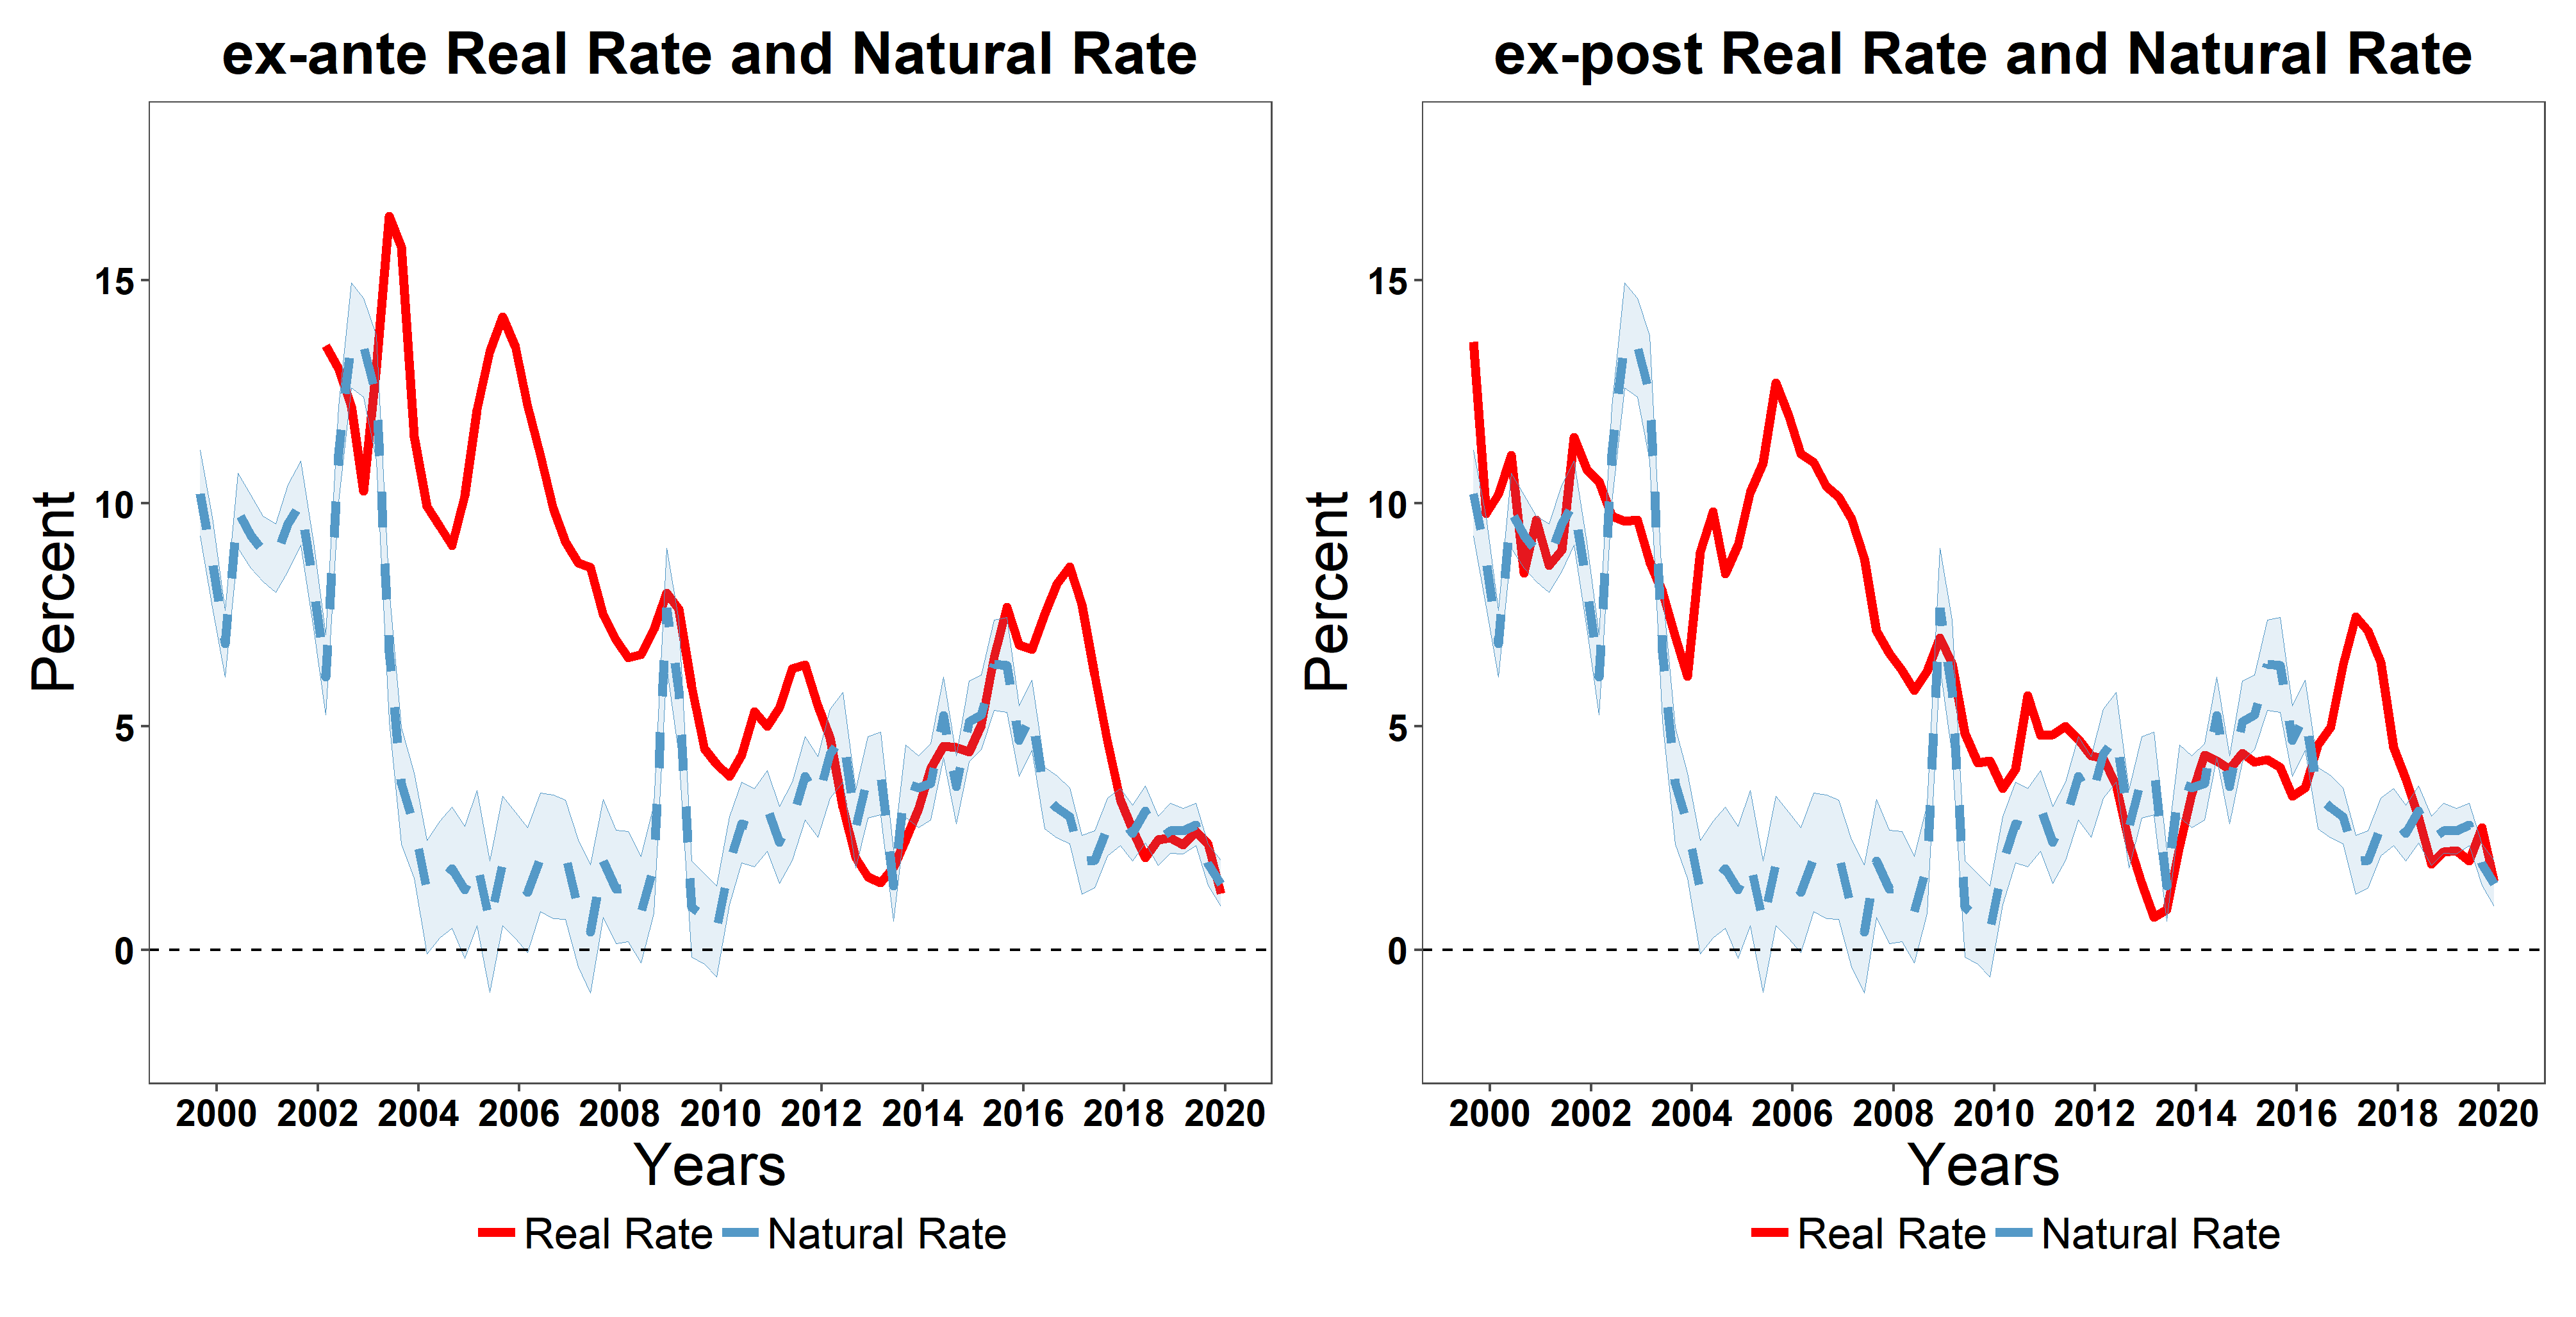
\includegraphics[scale=0.52]{Capitulo_1/Juros_Natural_Juros_Real.png}
\end{center}
\fnote{\small Note: The dashed line is the posterior mean and the shaded areas represent the 90\% confidence intervals of the estimate. The natural rate was computed using the DSGE model.}
\end{figure}

The first thing to note is that the natural rate shows considerable fluctuation over time, varying between 1.47\% to 13.70\% and average 4.16\% per annum. This movement is a characteristic of the neutral interest estimates using DSGE models according to  \citet{Justiniano:2010} and \citet{DelNegro:2017}. The second point is that the natural rate estimate follows a downward trend in the last twenty years, a result similar to that found in advanced economies, such as \citet{Melosi:2015}, \citet{Hristov:2016}, \citet{Okazaki:2018} and \citet{Neri:2018}. It is also observed in emerging economies, such as in Turkey, as \citet{Us:2018} pointed out.

The peak in estimates of natural interest was in the third quarter of 2002. This period coincides with the presidential elections associated with a possible victory by the then-presidential candidate, which was more radical at that time. The result was a crisis of confidence, which caused an exchange rate depreciation and increased country risk. After the elections, with the dissipation of that risk, natural interest rates dropped sharply. However, real interest did not follow this decline; on the contrary, throughout the 2000s, neutral interest was below real interest (either ex-ante or ex-post), indicating a  monetary policy tightening. And after the GFC, the BCB reduced interest rates to below neutral to stimulate the economy. Even so, in the middle of the decade of 2010, this situation was reversed to real interest rates above neutral. Since 2017, natural interest has been lower than its historical average.
\\
\\

\textbf{The stance of the monetary policy} \\

The Figure \ref{fig:Interest_gap} presents the smoothed mean measures of the real interest rate gap calculated by the difference between the real ex-ante rate and the natural rate. The interest gap is usually used as a measure of the monetary policy stance. If the interest gap is positive, this indicates that the monetary policy stance was conservative to reduce inflationary pressures and the output gap is negative. On the other hand, if the interest gap is negative, the monetary policy stance was expansionary, allowing for an increase in inflation and a positive output gap.\footnote{If the central banker could determine short-term interest equal to equilibrium interest, the output would reach its maximum level. That is, the output gap would be equal to zero (close the output gap). The difficulty here is to close the interest gap, as we have not observed natural interest, as it is a latent variable.}


\begin{figure}[H]
\begin{center}
\caption{Real interest rate gap}
\label{fig:Interest_gap}
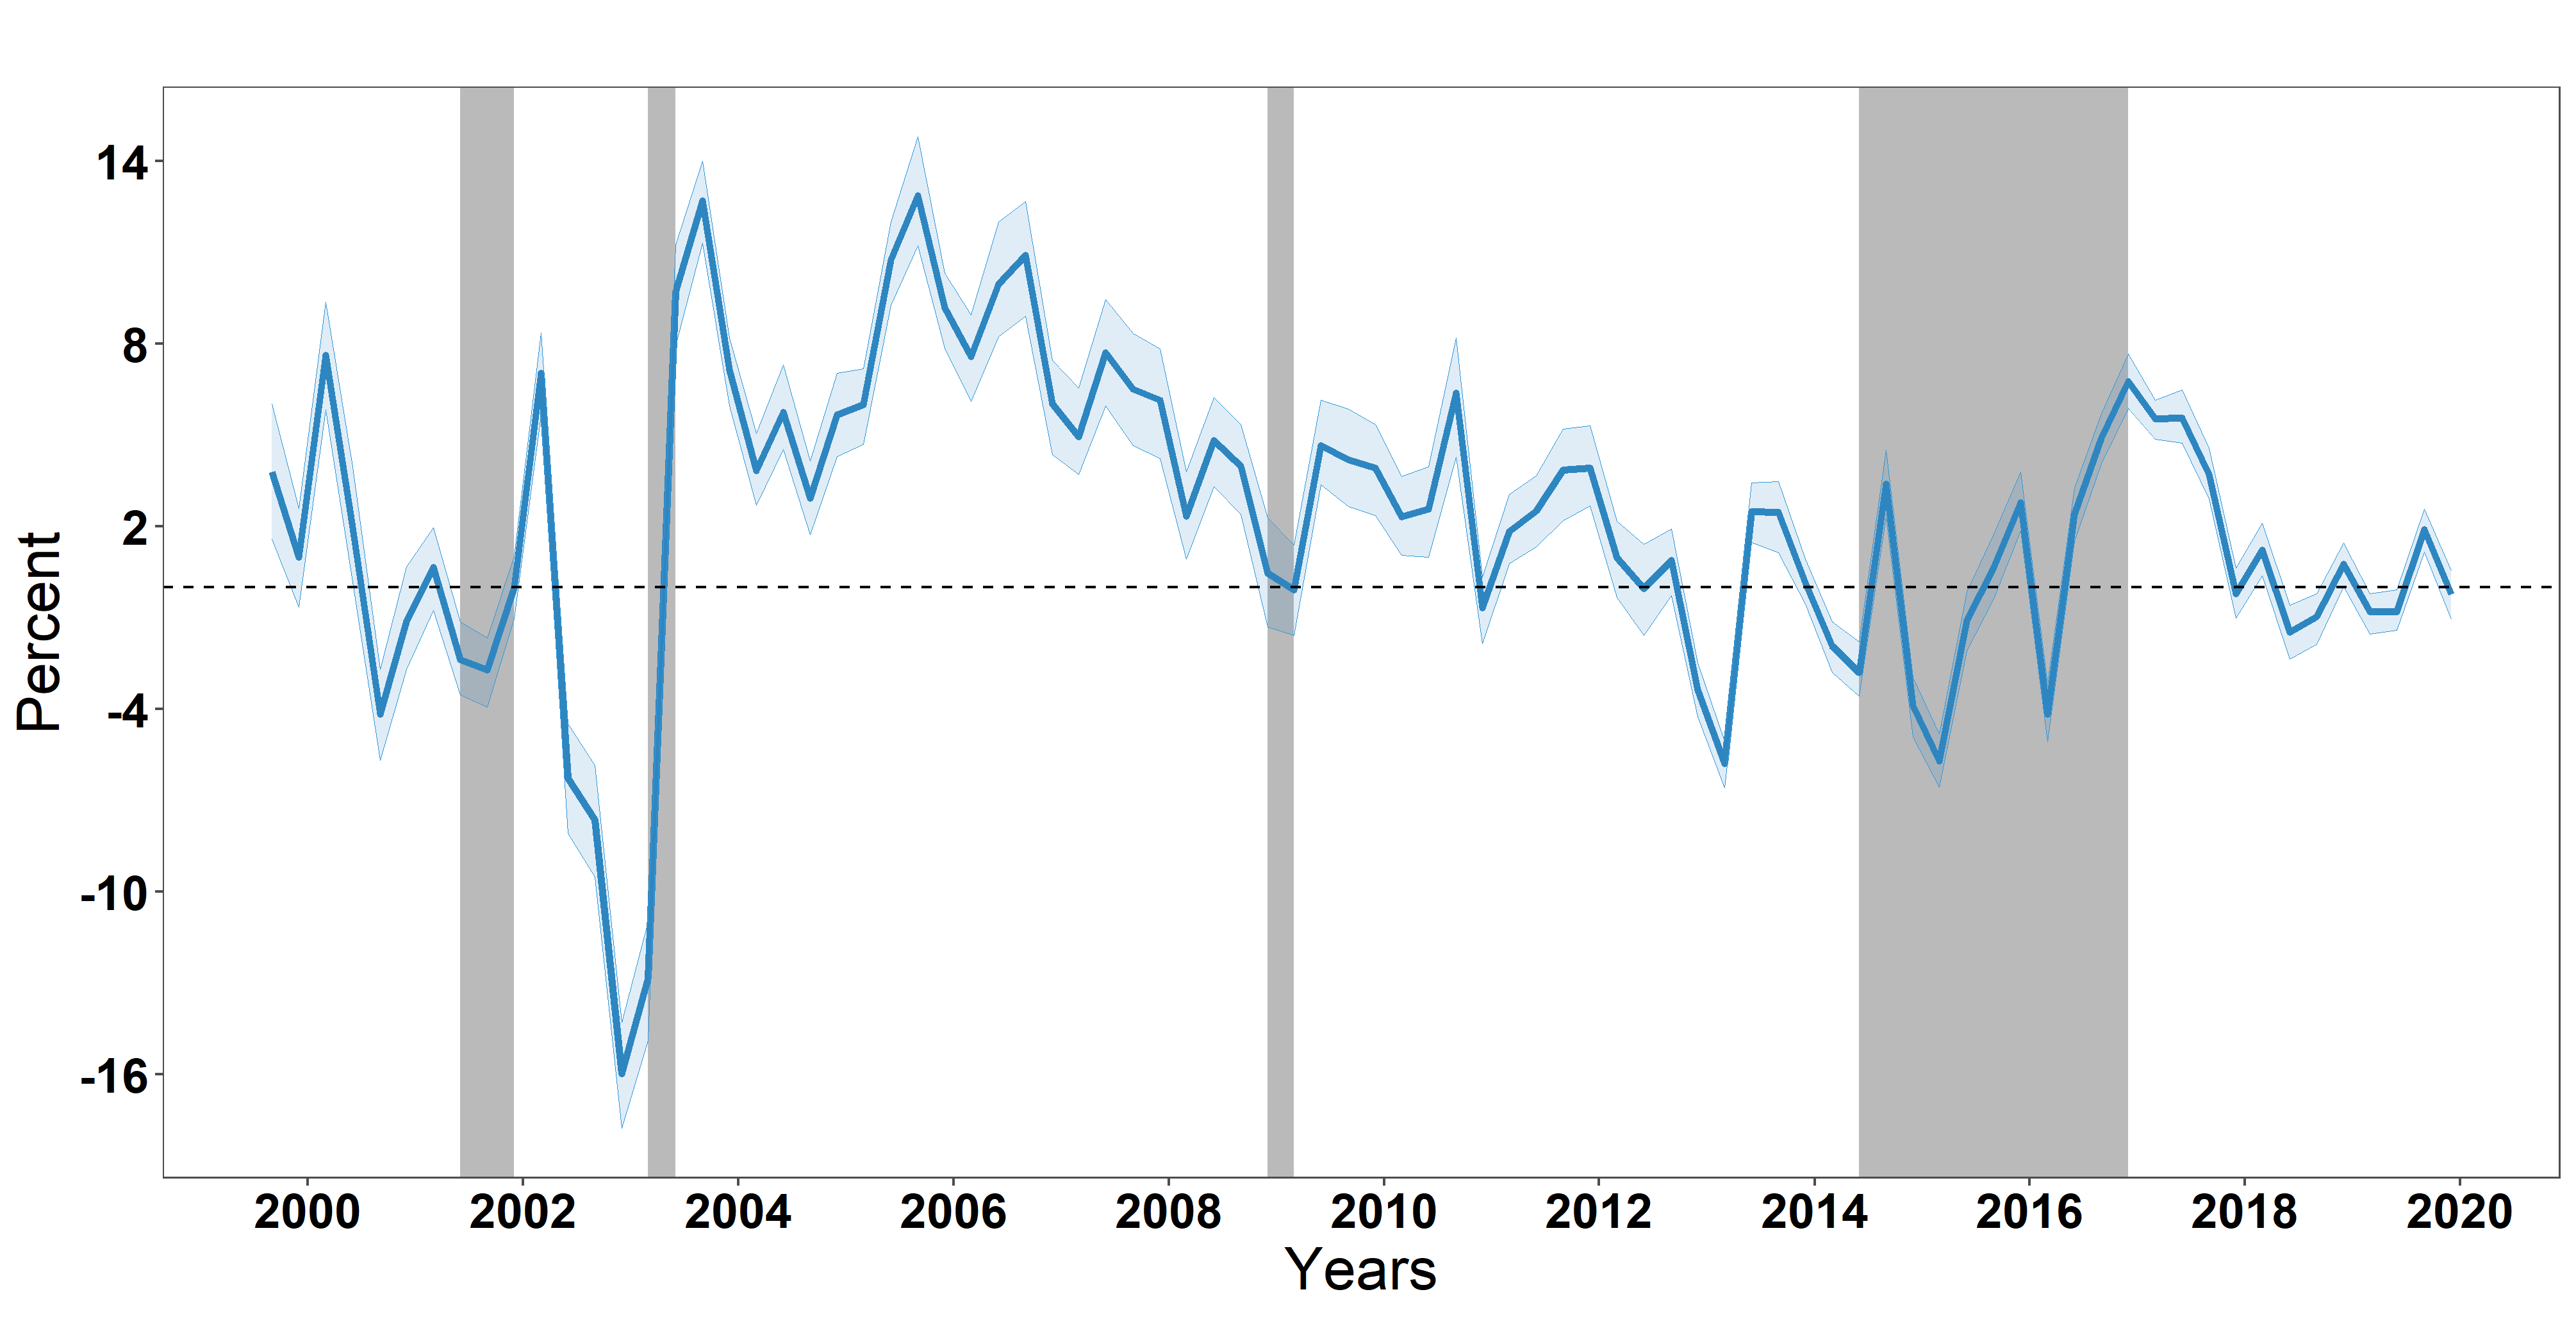
\includegraphics[scale=0.50]{Capitulo_1/GAP_Juros.png}    
\end{center}
\fnote{\small Note: The solid blue line is the short-term real interest rate gap. The light-blue shaded regions represent the 90\% confidence intervals of the estimate. Gray vertical shared areas indicate recession dates as measured by the Brazilian Business Cycle Dating Committee (CODACE).}
\end{figure}

The interest gap estimate shows that the gap was positive for more quarters, indicating that monetary policy has been predominantly contractionary in the last twenty years. The negative interest gap coincided with periods of recession in most quarters, suggesting that the BCB used monetary policy to stimulate the economy. From the beginning of the 2000s until the GFC, the interest gap was predominantly positive, indicating a tightening of monetary policy due to the recent history of inflation in Brazil.

The first half of the decade of 2010 was marked by the reduction of the interest gap through a monetary loosening, resulting in negative gap quarters. It was also when Brazilian inflation was above the target center, and inflation expectations were disanchored. Still, in 2014, there is a return to the tightening of monetary policy to reduce inflation and anchor inflation expectations at the target's center. In the most recent years, there was a decrease in the interest gap. Even with the control of inflation and the economic activity still in slow recovery, the BCB returned with the monetary easing. For this reason, the interest gap has closed. 
\\

\textbf{The forward rates} \\

The natural rate obtained using DSGE models is the estimate of short-term equilibrium interest. In the same way as the interest gap. The path of future expectations of the short-term interest gap is fundamental for determining inflation and output. The long-term interest gap provides information on current and expected interest, inflation, and natural interest rates. From this perspective in mind, we will follow \citet{Justiniano:2010} and \citet{DelNegro:2017} and we estimate the forward natural real rate and the forward ex-ante real rate.

\begin{figure}[H]
\begin{center}
\caption{The Forward Real Interest Rate $E_t(r_{t+h})$ and
Forward Natural Real Interest Rate $E_t(r_{t+h}^{n})$}
\label{fig:Forward_rate}
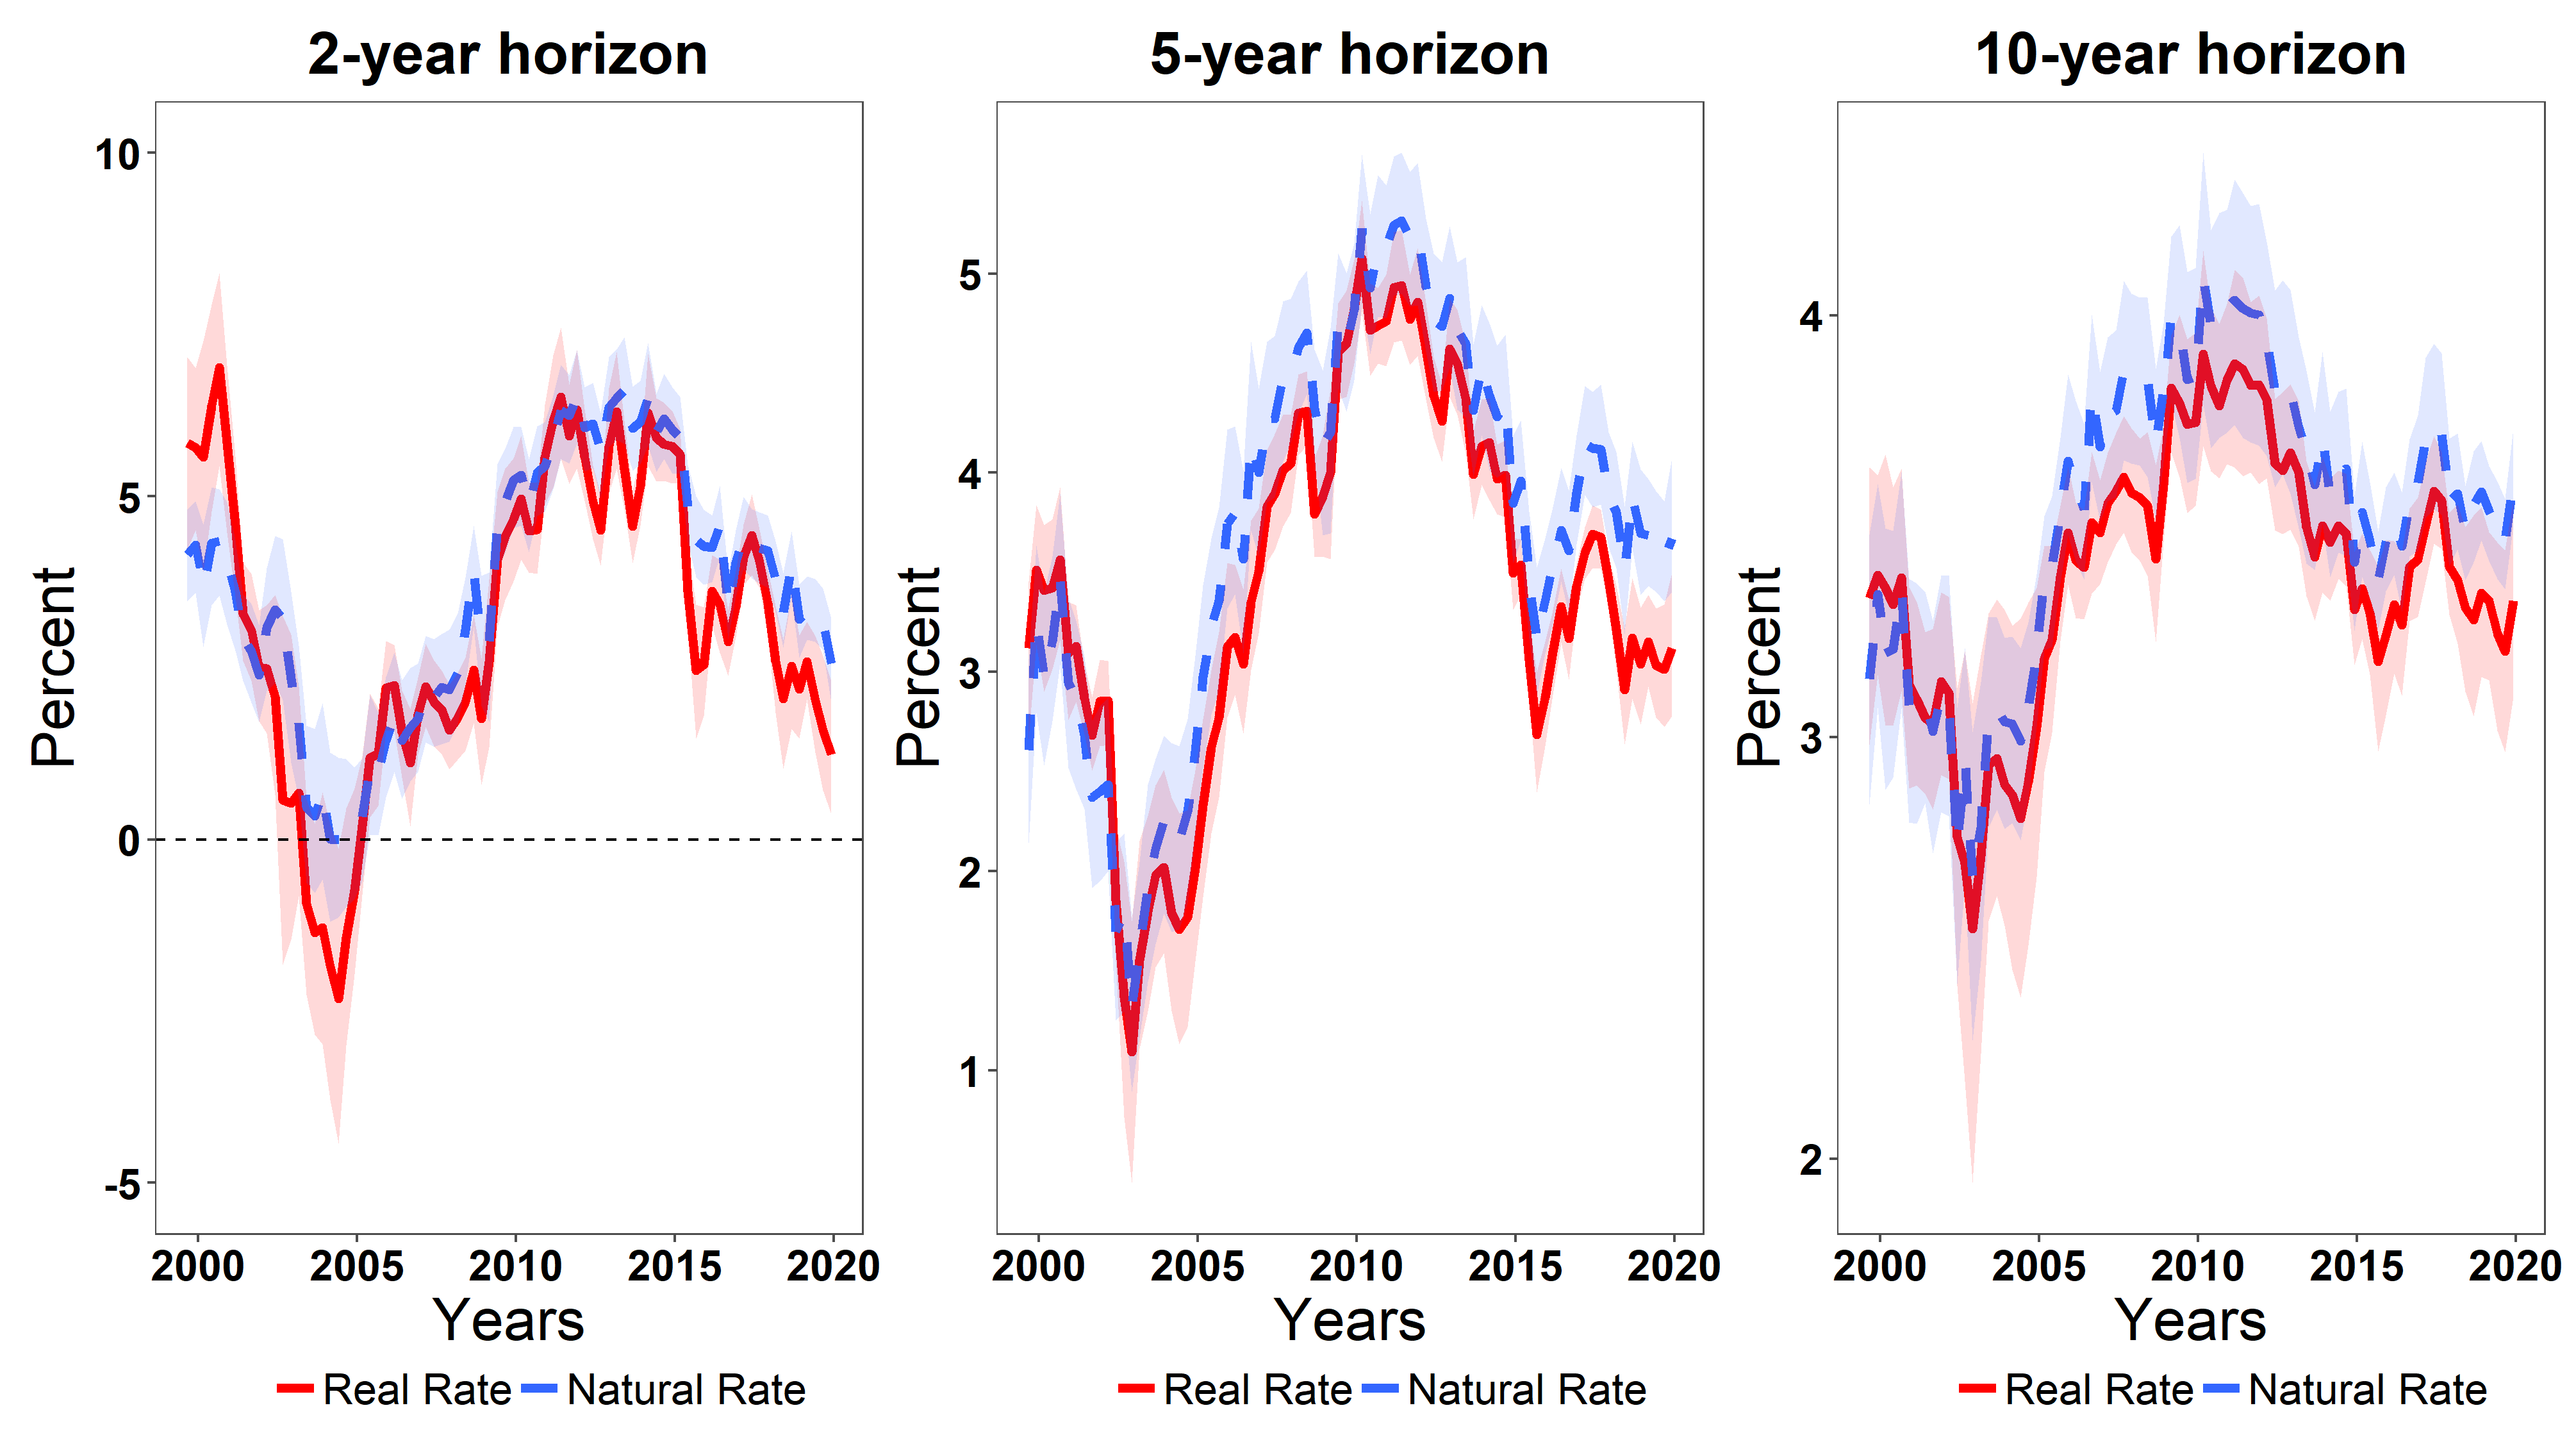
\includegraphics[scale=0.52]{Capitulo_1/Juros_Forward.png}  
\end{center}
\fnote{\small Note: The solid and dashed line are the posterior mean. The light blue and red shaded regions represent the 90\% confidence intervals of the estimates. }
\end{figure}


Figure (\ref{fig:Forward_rate}) illustrates real interest and the natural rate forecasts for 8, 20, and 40 quarters.\footnote{We will refer to the forward rate of these interest forecasts.} The two series move together across the three horizons. Even for a long-term forecast based on a DSGE model, the two forward rates fluctuate considerably. This result is similar to that found by \citet{DelNegro:2017}. 

The forward natural interest rate is higher than the forward ex-ante real interest rate in the three horizons (except for a few quarters over the 2-year horizon). For this reason, the long-term interest gap is negative for the most of the quarters. There is a tendency to grow the two forward rates, starting in 2004, in the three horizons. However, beginning in 2010, there is a downward trend. The forward natural rate and the forward real rate for 20 and 40 quarters appear to converge to a long-term steady-state value between 3\% and 4\%.



%%%%%%%%%%%%%%%%%%%%%%%%
%%%%%%%%%%%%%%%%%%%%%%%%
\subsection{Impulse Response Functions to Fundamental Shocks}
\subsection{Shock Decomposition}
\subsection{Driving forces}
%%%%%%%%%%%%%%%%%%%%%%%%
%%%%%%%%%%%%%%%%%%%%%%%%
\section{Sensitivity Analysis}
















\nocite{Palma:2014}
\nocite{Gali:2005}
\nocite{Lubik:2007}
\nocite{Carvalho:2015}
\nocite{Preston:2010}
\nocite{Monacelli:2005}
\nocite{Adolfson:2007}
\nocite{Adolfson:2008}
\nocite{Adolfson:2011}
\nocite{Altig:2011}
\nocite{Christiano:2011}
\nocite{Smets:2003}
\nocite{Smets:2007}
\nocite{Castro:2015}
\nocite{Christiano:2005}
\nocite{Woodford:2003}
\nocite{Gali:2015}
\nocite{Bernhardsen:2007}
\nocite{Brand:2018}
\nocite{Taylor:1993}



%
%
\bibliographystyle{apalike}
\bibliography{Bibliografia}
%%%%%%%%%%%%
%%%%%%%%%%%%

\section*{Appendix I: The Linearised Model}

\subsection*{Firms}

%%%%%%%%%%%%%%%%%
%%%%%%%%%%%%%%%%%
\subsubsection*{Domestic goods}

Production
\begin{equation}
    \hat{y}_{t}=\lambda^{d}\left(\hat{\varepsilon}_{t}+\alpha\left(\hat{k}_{t}-\hat{\mu}_{t}^{z}\right)+(1-\alpha) \hat{H}_{t}\right)
\end{equation}

Rental rate of capital
\begin{equation}
    \hat{r}_{t}^{k}=\hat{w}_{t}+\hat{\mu}_{t}^{z} + \hat{R}_t^{f}-\hat{k}_{t}+\hat{H}_{t}
\end{equation}

The New Keynesian Phillips Curve
\begin{equation}
     \begin{aligned}
    \hat{\pi}_{t}^{d}-\hat{\tilde{\pi}}_{t}^{c} &=\frac{\beta}{1+\beta \kappa_{d}}\left(E_{t} \hat{\pi}_{t+1}^{d}-\rho_{\pi} \hat{\bar{\pi}}_{t}^{c}\right)+\frac{\kappa_{d}}{1+\beta \kappa_{d}}\left(\hat{\pi}_{t-1}^{d}-\hat{\tilde{\pi}}_{t}^{c}\right)-\frac{\beta \kappa_{d}\left(1-\rho_{\pi}\right)}{1+\beta \kappa_{d}} \hat{\bar{\pi}}_{t}^{c} \\
    &+\frac{\left(1-\theta_{d}\right)\left(1-\beta \xi_{d}\right)}{\left(1+\beta \kappa_{d}\right) \xi_{d}}\left(\hat{m} c_{t}^{d}+\hat{\lambda}_{t}^{d}\right)
    \end{aligned} 
\end{equation}

The real marginal cost
\begin{equation}
\begin{aligned}
\hat{m} c_{t}^{d} &=\alpha \hat{r}_{t}^{k}+(1-\alpha)\left[\widehat{\bar{w}}_{t}+\hat{R}_{t}^{f}\right]-\hat{\varepsilon}_{t} \\
&=\alpha\left(\hat{\mu}_{t}^{z}+\hat{H}_{t}-\hat{k}_{t}\right)+\widehat{\bar{w}}_{t}+\hat{R}_{t}^{f}-\hat{\varepsilon}_{t}
\end{aligned}
\end{equation}

%%%%%%%%%%%%%%%%%
%%%%%%%%%%%%%%%%%
\subsubsection*{Imported goods}

The New Keynesian Phillips curve of imported consumption and investment goods
\begin{equation}
    \begin{aligned}
    \hat{\pi}_{t}^{m, c}-\hat{\bar{\pi}}_{t}^{c} &=\frac{\beta}{1+\beta \kappa_{m, c}}\left(E_{t} \hat{\pi}_{t+1}^{m, c}-\rho_{\pi} \hat{\bar{\pi}}_{t}^{c}\right)+\frac{\kappa_{m, c}}{1+\beta \kappa_{m, c}}\left(\hat{\pi}_{t-1}^{m, c}-\hat{\bar{\pi}}_{t}^{c}\right)-\frac{\kappa_{m, c} \beta\left(1-\rho_{\pi}\right)}{1+\beta \kappa_{m, c}} \hat{\bar{\pi}}_{t}^{c} \\
    &+\frac{\left(1-\xi_{m, c}\right)\left(1-\beta \xi_{m, c}\right)}{\left(1+\beta \kappa_{m, c}\right) \xi_{m, c}}\left(\hat{m} c_{t}^{m, c}+\hat{\lambda}_{t}^{m, c}\right)
    \end{aligned}
\end{equation}

\begin{equation}
     \begin{aligned}
    \hat{\pi}_{t}^{m, i}-\hat{\bar{\pi}}_{t}^{c} &=+\frac{\beta}{1+\beta \kappa_{m, i}}\left(E_{t} \hat{\pi}_{t+1}^{m, i}-\rho_{\pi} \hat{\bar{\pi}}_{t}^{c}\right)+\frac{\kappa_{m, i}}{1+\beta \kappa_{m, i}}\left(\hat{\pi}_{t-1}^{m, i}-\hat{\bar{\pi}}_{t}^{c}\right)-\frac{\kappa_{m, i} \beta\left(1-\rho_{\pi}\right)}{1+\beta \kappa_{m, i}} \hat{\bar{\pi}}_{t}^{c} \\
    &+\frac{\left(1-xi_{m, i}\right)\left(1-\beta \xi_{m, i}\right)}{\left(1+\beta x_{m, i}\right) \xi_{m, i}}\left(\hat{m} c_{t}^{m, i}+\hat{\lambda}_{t}^{m, i}\right)
    \end{aligned}
\end{equation}

The marginal costs for consumption and investment good importers

\begin{equation}
    \widehat{m c}_{t}^{m, c}=-\widehat{m c}_{t}^{x}-\hat{\gamma}_{t}^{x, *}-\hat{\gamma}_{t}^{m c, d}
\end{equation}

\begin{equation}
    \widehat{m c}_{t}^{m, i}=-\widehat{m c}_{t}^{x}-\hat{\gamma}_{t}^{x, *}-\hat{\gamma}_{t}^{m i, d}
\end{equation}

%%%%%%%%%%%%%%%%%
%%%%%%%%%%%%%%%%%
\subsubsection*{Exported goods}
The New Keynesian Phillips curve of exported goods

\begin{equation}
    \begin{aligned}
\hat{\pi}_{t}^{x} - \hat{\bar{\pi}}_{t}^{c} &=\frac{\beta}{1+\beta \kappa_{x}}\left(E_{t} \hat{\pi}_{t+1}^{x}-\rho_{\pi} \hat{\pi}_{t}^{c}\right)+\frac{\kappa_{x}}{1+\beta x_{x}}\left(\hat{\pi}_{t-1}^{x}-\hat{\bar{\pi}}_{t}^{c}\right)-\frac{\kappa_{x} \beta\left(1-\rho_{\pi}\right)}{1+\beta \kappa_{x}} \hat{\bar{\pi}}_{t}^{c} \\
&+\frac{\left(1-\xi_{x}\right)\left(1-\beta \xi_{x}\right)}{\left(1+\beta \kappa_{x}\right) \xi_{x}}\left(\hat{m} c_{t}^{x}+\hat{\lambda}_{t}^{x}\right)
\end{aligned}
\end{equation}

The marginal costs for exported goods
\begin{equation}
    \hat{m} c_{t}^{x}=\hat{m} c_{t-1}^{x}+\hat{\pi}_{t}^{d}-\hat{\pi}_{t}^{x}-\Delta \hat{S}_{t}
\end{equation}

%%%%%%%%%%%%%%%%%
%%%%%%%%%%%%%%%%%
\subsection*{Households}

Consumption Euler equation
\begin{equation}
    \begin{aligned}
\hat{c}_{t} &=\frac{\mu^{z} b}{\left(\mu^{z}\right)^{2}+\beta b^{2}} \hat{c}_{t-1}+\frac{\beta \mu^{z} b}{\left(\mu^{z}\right)^{2}+\beta b^{2}} E_{t} \hat{c}_{t+1}-\frac{\mu^{z} b}{\left(\mu^{z}\right)^{2}+\beta b^{2}}\left(\hat{\mu}_{t}^{z}-\beta E_{t} \hat{\mu}_{t+1}^{z}\right) \\
&-\frac{\left(\mu^{z}-b\right)\left(\mu^{z}-\beta b\right)}{\left(\mu^{z}\right)^{2}+\beta b^{2}}\left(\hat{\psi}_{t}^{z}+\hat{\gamma}_{t}^{c, d}\right)+\frac{\mu^{z}-b}{\left(\mu^{z}\right)^{2}+\beta b^{2}}\left(\mu^{z} \hat{\xi}_{t}^{c}-\beta b E_{t} \hat{\zeta}_{t+1}^{c}\right)
\end{aligned}
\end{equation}

Real wage
\begin{equation}
\label{labor_wage_equation}    \hat{w}_{t}=-\frac{1}{\eta_{1}}\left[\begin{array}{l}
    \eta_{0} \hat{w}_{t-1}+\eta_{2} E_{t} \hat{w}_{t+1}+\eta_{3}\left(\hat{\pi}_{t}^{d}-\hat{\tilde{\pi}}_{t}^{c}\right)+\eta_{4}\left(E_{t} \hat{\pi}_{t+1}^{d}-\rho_{\pi} \hat{\tilde{\tau}}_{t}^{c}\right) \\
    +\eta_{5}\left(\hat{\pi}_{t-1}^{c}-\hat{\tilde{\pi}}_{t}^{c}\right)+\eta_{6}\left(\hat{\pi}_{t}^{c}-\rho_{\pi} \hat{\tilde{\pi}}_{t}^{c}\right)+\eta_{7} \hat{\psi}_{t}^{z}+\eta_{8} \hat{H}_{t}+\eta_{9} \zeta_{t}^{h}
    \end{array}\right]
\end{equation}

Parameters in Equation (\ref{labor_wage_equation}) are defined as follows:
$$b_{w}=\frac{\lambda_{w} \sigma_{L}-\left(1-\lambda_{w}\right)}{\left(1-\beta \xi_{w}\right)\left(1-\xi_{w}\right)},$$

$$
\left(\begin{array}{c}
\eta_{0} \\
\eta_{1} \\
\eta_{2} \\
\eta_{3} \\
\eta_{4} \\
\eta_{5} \\
\eta_{6} \\
\eta_{7} \\
\eta_{8} \\
\eta_{9}
\end{array}\right)=\left(\begin{array}{c}
b_{w} \xi_{w} \\
\lambda_{w} \sigma_{L}-b_{w}\left(1+\beta \xi_{w}^{2} \right) \\
b_{w} \beta \xi_{w} \\
-b_{w} \xi_{w} \\
b_{w} \beta \xi_{w} \\
b_{w} \xi_{w} \kappa_{w} \\
-b_{w} \beta \xi_{w} \kappa_{w} \\
\left(1-\lambda_{w}\right) \\
-\left(1-\lambda_{w}\right) \sigma_{L} \\
-\left(1-\lambda_{w}\right)
\end{array}\right)
$$

The equilibrium condition for investment
\begin{equation}
    \hat{i}_{t}=\frac{1}{1+\beta}\left[\beta E_{t} \hat{i}_{t+1}+\hat{i}_{t-1}+\beta E_{t} \hat{\mu}_{t+1}^{z}-\mu_{t}^{z}\right]+\frac{1}{\left(\mu^{z}\right)^{2} \phi_{i}(1+\beta)}\left(\hat{P}_{t}^{k}-\hat{\gamma}_{t}^{i, d}+\hat{\zeta}_{t}^{i}\right)
\end{equation}

Price of installed capital
\begin{equation}
    \hat{P}_{t}^{k}=E_{t}\left[\frac{(1-\delta) \beta}{\mu^{z}} \hat{P}_{t+1}^{k}+\hat{\psi}_{t+1}^{2}-\hat{\psi}_{t}^{z}-\hat{\mu}_{t+1}^{z}+\frac{\mu^{z}-(1-\delta) \beta}{\mu^{z}} \hat{r}_{t+1}^{k}\right]
\end{equation}

The Capital’s law-of-motion:

\begin{equation}
    \hat{\bar{k}}_{t+1}=\frac{1-\delta}{\mu^{z}}\left(\hat{\bar{k}}_{t}-\hat{\mu}_{t}^{z}\right)+\left(1-\frac{1-\delta}{\mu^{z}}\right)\left(\hat{i}_{t}+\hat{\zeta}_{t}^{i}\right)
\end{equation}

The capital utilization

\begin{equation}
     \hat{u}_{t}=\frac{1}{\sigma_{a}} \hat{r}_{t}^{k}
\end{equation}


The capital services is

\begin{equation}
    \hat{k}_{t}=\hat{\bar{k}}_{t}+\hat{u}_{t}
\end{equation}

The risk premium-adjusted uncovered interest rate parity
condition

\begin{equation}
    \hat{R}_{t}-\hat{R}_{t}^{*}&=&\left(1-\tilde{\phi}_{s}\right) E_{t} \Delta \hat{S}_{t+1}-\tilde{\phi}_{s} \Delta \hat{S}_{t}-\tilde{\phi}_{a} \hat{a}_{t}+\hat{\tilde{\phi}}_{t}
\end{equation}

%%%%%%%%%%%%%%%%%
%%%%%%%%%%%%%%%%%
\subsection*{The Central Bank}
Taylor rule

\begin{equation}
\begin{aligned}
\hat{R}_{t}=& \rho_{R} \hat{R}_{t-1}+(1-\rho_{R})\left\{\hat{\bar{\pi}}_{t}^{c}+\phi_{\pi}\left(\hat{\pi}_{t+1}^{c}-\hat{\bar{\pi}}_{t}^{c}\right)+\phi_{y}\left(\hat{Y}_{t}-\hat{Y}_{t}^{n}\right) + \phi_{x}\hat{x}_{t-1}\right\} + \varepsilon_{t}^{R}
\end{aligned}
\end{equation}

The CPI inflation measure 

\begin{equation}
      \hat{\pi}_{t}^{c}=\left(1-\vartheta_{c}\right)\left(\frac{1}{\gamma^{c, d}}\right)^{1-\eta_{\epsilon}} \hat{\pi}_{t}^{d}+\vartheta_{c}\left(\gamma^{m c, c}\right)^{1-\eta_{c}} \hat{\pi}_{t}^{m, c}
\end{equation}

%%%%%%%%%%%%%%%%%
%%%%%%%%%%%%%%%%%
\subsection*{Relative prices}

The consumption and investment goods:
\begin{equation}
    \hat{\gamma}_{t}^{c, d} &=\hat{\gamma}_{t-1}^{i, d}+\hat{\pi}_{t}^{c}-\hat{\pi}_{t}^{d} 
\end{equation}

\begin{equation}
      \hat{\gamma}_{t}^{i, d} &=\hat{\gamma}_{t-1}^{i, d}+\hat{\pi}_{t}^{i}-\hat{\pi}_{t}^{d}
\end{equation}

The imported consumption and investment goods:
\begin{equation}
    \hat{\gamma}_{t}^{m c, d}=\hat{\gamma}_{t-1}^{m c, d}+\hat{\pi}_{t}^{m, c}-\hat{\pi}_{t}^{d}
\end{equation}

\begin{equation}
      \hat{\gamma}_{t}^{m i, d}=\hat{\gamma}_{t-1}^{m i, d}+\hat{\pi}_{t}^{m, i}-\hat{\pi}_{t}^{d}
\end{equation}

Export goods
\begin{equation}
      \hat{\gamma}_{t}^{x, *}=\hat{\gamma}_{t-1}^{x, *}+\hat{\pi}_{t}^{x}-\hat{\pi}_{t}^{*}
\end{equation}

The real exchange rate:
\begin{equation}
      \hat{\gamma}_{t}^{s}=-\omega_{c}\left(\frac{1}{\gamma^{m c, c}}\right)^{\eta_{c}-1} \hat{\gamma}_{t}^{m c, d}-\hat{\gamma}_{t}^{x, *}-\hat{m} c_{t}^{x}
\end{equation}

%%%%%%%%%%%%%%%%%
%%%%%%%%%%%%%%%%%
\subsection*{Market Clearing}
Domestic goods market
\begin{equation}
    \begin{aligned}
    \hat{y}_{t} &=\left(1-\omega_{c}\right)\left(\gamma^{c, d}\right)^{\eta_{c}} \frac{c}{y}\left(\hat{c}_{t}+\eta_{c} \hat{\gamma}_{t}^{c, d}\right)+\left(1-\omega_{i}\right)\left(\gamma^{i, d}\right)^{\eta_{i}} \frac{i}{y}\left(\hat{i}_{t}+\eta_{i} \hat{\gamma}_{t}^{i, d}\right) \\
    &+g_{y} \hat{g}_{t}+\frac{y^{*}}{y}\left(\hat{y}_{t}^{*}-\eta_{f} \hat{\gamma}_{t}^{x, *}+\hat{z}_{t}^{*}\right)+\frac{r^{k}}{\mu^{z}} \frac{k}{y}\left(\hat{k}_{t}-\hat{\bar{k}}_{t}\right)
    \end{aligned}
\end{equation}

The law of motion for net foreign assets
\begin{equation}
      \begin{aligned}
    \hat{a}_{t} &=-y^{*} \hat{m} c_{t}^{x}-\eta_{f} y^{*} \hat{\gamma}_{t}^{x, *}+y^{*} \hat{y}_{t}^{*}+y^{*} \hat{z}_{t}^{*}+\left(c^{m}+i^{m}\right) \hat{\gamma}_{t}^{f} \\
    &-\left[c^{m}\left(-\eta_{c}\left(1-\omega_{c}\right)\left(\gamma^{c, d}\right)^{\eta_{c}-1}\right) \hat{\gamma}_{t}^{m c, d}+\hat{c}_{t}\right] \\
    &-\left[i^{m}\left(-\eta_{i}\left(1-\omega_{i}\right)\left(\gamma^{i, d}\right)^{\eta_{i}-1}\right) \hat{\gamma}_{t}^{m i, d}+\hat{i}_{t}\right] 
    +\frac{\pi^{*}}{\pi} \frac{1}{\beta} \hat{a}_{t-1}
    \end{aligned}
\end{equation}


%
%
\end{document}

